% !TEX root = ../Thesis.tex
% !TEX output_directory
\documentclass[11pt,a4paper,english,greek,twoside]{../Thesis}
\begin{document}
\chapter{Σημασιολογικό Υποσύστημα: Αντικείμενα} \label{chap:Experiments}
Στο κεφάλαιο 2 είδαμε τη σημασία της σημασιολογίας στην αναγνώριση δράσεων. Παρότι οι προσεγγίσεις που βασίζονται σε αυτή είναι συχνά εξαρτημένες από συνύπαρξη με μεθόδους χαρακτηριστικών χαμηλού επιπέδου, η συνεισφορά τους με την υψηλού επιπέδου αναπαράσταση των δράσεων στην εκτίμηση αυτών είναι καίρια. Σε αυτή την εργασία αναζητάμε σημασιολογικά χαρακτηριστικά μέσω αντικειμένων και τύπων λαβής. Σε αυτό το κεφάλαιο ασχολούμαστε μόνο με τη σημασία των αντικειμένων και αφήνουμε για επόμενο κεφάλαιο την ανάλυση των τύπων λαβής. Η οργάνωση του κεφαλαίου έχει ως εξής: αρχίζουμε με ιστορική αναφορά στις μεθόδους ανίχνευσης αντικειμένων και εύρεσης προσκηνίου. Ακολουθεί το θεωρητικό υπόβαθρο των μεθόδων που αξιοποιούμε (Ταίριασμα Προτύπων, εξαγωγή προσκηνίου με Γκαουσιανά Μοντέλα Μίξης, ανιχνευτής ανθρώπων με χρήση Μοντέλων Παραμορφώσιμων Τμημάτων) και αναλύουμε εκτενώς τις σχεδιαστικές μας επιλογές. Κλείνουμε με ένα σχόλιο πάνω στη θαυμαστή συνθετότητα της ανθρώπινης αντίληψης στο πρόβλημα της ανίχνευσης και ταυτοποίησης αντικειμένων.


%%%%%%%%%%%%%%%%%%%%%%%%%%%%%%%%%%%%%%%%%%%%% Object Detection
\section{Ανίχνευση Αντικειμένων σε Εικόνες}
%%%%%%%%%%%%%%%%%%%%%%%% General
\subsection{Γενικά}
Η ανίχνευση αντικειμένων είναι ένα σημαντικό και δύσκολο πρόβλημα της Όρασης Υπολογιστών. Όπως δηλώνει το όνομά της, το ζήτημα είναι ο χωρικός εντοπισμός της εμφάνισης μιας κλάσης μέσα σε μια εικόνα και μπορεί να διατυπωθεί μαθηματικά ως εξής: Δοθείσας μιας εικόνας και μιας κατηγορίας αντικειμένων, να βρεθεί η ελάχιστη σε εμβαδόν περιοχή, η οποία περικλείει όλο το αντικείμενο. Η περιοχή αυτή μπορεί να έχει αυθαίρετο σχήμα, να ταυτίζεται με το σχήμα του αντικειμένου, όπως στην περίπτωση της κατάτμησης, αλλά συχνά επιλέγεται το ελάχιστο ορθογώνιο με την παραπάνω ιδιότητα. Οπότε ένα σύστημα ανίχνευσης αντικειμένου πρέπει να λάβει δύο αποφάσεις: αφενός να αποφασίσει για την εμφάνιση ή μη του ζητούμενου αντικειμένου στην εικόνα και αφετέρου να επιστρέψει την περιοχή εμφάνισης. Η τελευταία είναι και η ειδοποιός διαφορά από τα συστήματα ταυτοποίησης αντικειμένων τα οποία επιστρέφουν ως έξοδο μια προκαθορισμένη αριθμητική ή λογική τιμή ή ένα κατηγόρημα.

\par Η σημασία της δυνατότητας ανίχνευσης αντικειμένων είναι σπουδαία, τόσο για ένα φυσικό ον, όπως ο άνθρωπος, αλλά και για εφαρμογές Όρασης Υπολογιστών. Θα σταθούμε κυρίως στη δεύτερη κατηγορία αλλά θα δούμε και περιπτώσεις που η ανθρώπινη ανάγκη εμπνέει την Τεχνητή Νοημοσύνη. Ξεκινάμε από εφαρμογές όπου η ανίχνευση αντικειμένων είναι αυτοσκοπός, όπως τα συστήματα επίβλεψης και ασφαλείας χώρων ή αυτόματου εντοπισμού αστεροειδών σε εικόνες διαστημικών τηλεσκοπίων και γενικά βιομηχανικά συστήματα \cite{hirano_2006}. Περαιτέρω, η ανίχνευση αντικειμένων μπορεί να υποβοηθήσει την κατηγοριοποίησή τους, ενώ μπορεί ακόμα να συνεισφέρει στη σημασιολογική αντίληψη ενός χώρου. Τέλος, ο άνθρωπος χρειάζεται να εντοπίζει αντικείμενα για να αλληλεπιδράσει μαζί τους ή να λάβει αποφάσεις. Ένα ρομπότ που θα μπορεί ιδανικά να εντοπίζει αντικείμενα στο χώρο κίνησής του θα είναι σε θέση να υποβοηθήσει τον άνθρωπο σε πτυχές της καθημερινότητάς του \cite{DBLP:journals/corr/LiHXYGA16}.

\begin{figure}
  \centering
  \noindent\makebox[\textwidth]{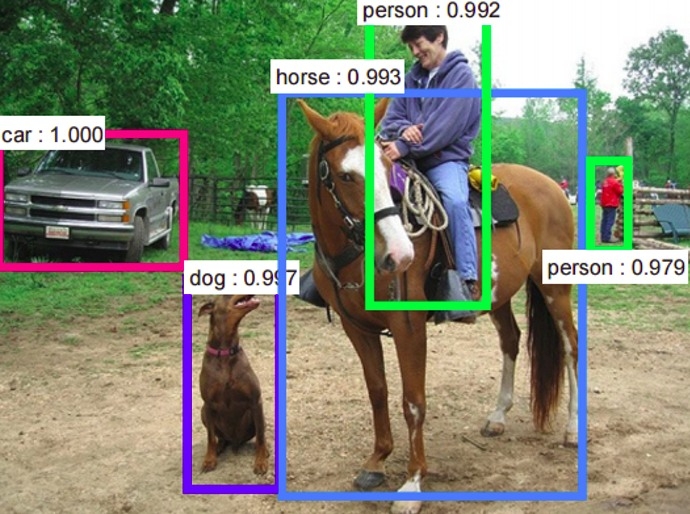
\includegraphics[scale=0.45]{{Images/chap4ObjDet}.jpg}}
  \caption{Παράδειγμα εξόδου συστήματος ανίχνευσης αντικειμένων. Βλέπουμε ότι το σύστημα μας επιστρέφει το ορθογώνιο στο οποίο εντοπίζεται το ζητούμενο αντικείμενο. Στα ορθογώνια επισημειώνεται επιπλέον το σκορ πεποίθησης του συστήματος για την ανίχνευση και ταυτοποίηση στην οποία προέβη. Εικόνα από το \cite{ren_2016}.}
  \label{fig:chap4ObjDet}
\end{figure}

\par Από την άλλη, η ανίχνευση αντικειμένων είναι ένα δύσκολο καθήκον για τους υπολογιστές, παρότι ταυτόχρονα είναι κάτι τετριμμένο για τους ανθρώπους \cite{pinto_2008}. Υπάρχουν πολλαπλά αίτια για αυτό το φαινόμενο. Θέματα όπως η αμεταβλητότητα στους γεωμετρικούς μετασχηματισμούς, στον φωτισμό, στις διαφορετικές όψεις του αντικειμένου, στις διαφορετικές αποστάσεις κάμερας και στις μερικές επικαλύψεις έχουν σε ικανοποιητικό βαθμό προβλεφθεί και μοντελοποιηθεί. Υπάρχουν όμως εγγενείς δυσκολίες στην ανίχνευση αντικειμένων, όπως η σημαντική ενδομεταβλητότητα μεταξύ αντικειμένων της ίδιας κλάσης, οι παραμορφώσεις των αντικειμένων και η αστάθεια στη φυσική τους υπόσταση (π.χ. ένα κρεμμύδι μπορεί να είναι ωμό, ακέραιο, μαγειρεμένο, τεμαχισμένο, τσιγαρισμένο και πάλι αντιπροσωπεύει την ίδια κλάση). Τέλος, ένα σύστημα οπτικής ανίχνευσης αντικειμένων χάνει τη σημασιολογική πληροφορία που οι άνθρωποι χρησιμοποιούν για να απαντήσουν στο ερώτημα εντοπισμού. Το ζήτημα αυτό αντιμετωπίζεται μερικώς με την αποδόμηση του αντικειμένου σε μικρότερες οντότητες, ωστόσο, συχνά το περιβάλλον και η χρήση είναι καταλληλότεροι παράγοντες απάντησης αλλά μοντελοποιούνται εξαιρετικά δύσκολα. Το σύνολο δεδομένων που χρησιμοποιούμε για τα πειράματά μας θα μας επιτρέψει στη συνέχεια να διαπιστώσουμε ορισμένους παράγοντες ανθρώπινης αντίληψης που σχετίζονται με την ανίχνευση αντικειμένων.


%%%%%%%%%%%%%%%%%%%%%%%% History
\subsection{Ιστορικά Στοιχεία}
Η σημασία του προβλήματος της ανίχνευσης αντικειμένων, σε συνδυασμό με τη δυσκολία επίλυσής του, ώθησαν πολυάριθμες και μακροχρόνιες ενασχολήσεις με διαφορετικές προσεγγίσεις και αποτελέσματα. Η ιστορία αυτών των προσπαθειών ξεκινά ήδη από το 1965, όταν ο Roberts \cite{roberts_1963} δημοσιεύει την πρωτοπόρα εργασία του, η οποία σηματοδοτεί την εποχή των γεωμετρικών προσεγγίσεων και της ευθυγράμμισης. Η γενική φιλοσοφία είναι η εύρεση σημείων τα οποία μας βοηθούν να αποφασίσουμε τον βέλτιστο μετασχηματισμό, συνήθως περιστροφή, μετάθεση και κλιμάκωση, ο οποίος θα ταυτίσει το πρότυπο που έχουμε για το αντικείμενο με αυτό που περιέχεται στην εικόνα \cite{huttenlocher_1987}. Η καθοριστική παραδοχή που γίνεται είναι η αμεταβλητότητα του αντικειμένου, το οποίο μπορεί να αναπαραστεί επιτυχώς από ένα προκαθορισμένο πρότυπο. Στο \cite{grimson_1987} χρησιμοποιούνται γεωμετρικά μοντέλα για την εύρεση μερικώς επικαλυπτόμενων αντικειμένων. Μάλιστα δίνεται έμφαση στη δύναμη των μοντέλων αυτών για την συρρίκνωση της περιοχής αναζήτησης. Το \cite{lozanoperez_1986} χρησιμοποιεί επιπλέον παραδοχές για το μετασχηματισμό ευθυγράμμισης έτσι ώστε με προεπεξεργασία να ελαττώσει το χρόνο ανίχνευσης. Μια ακόμα παραδοχή της εποχής είναι η ακαμψία των αντικειμένων, η οποία μπορεί να γίνει εκμεταλλεύσιμη στην γεωμετρική αναπαράσταση των αντικειμένων με γραμμές και επίπεδα \cite{faugeras_1986}. Η ανάγκη για αναισθησία στην οπτική γωνία παρακολούθησης του αντικειμένου εμφανίζεται αυτή την εποχή στο \cite{Lowe_1987}, το οποίο θίγει επίσης πιθανοτικά μοντέλα για ταχύτερο εντοπισμό περιοχών ενδιαφέροντος. Πριν κλείσουμε με το “ρεύμα” της ευθυγράμμισης και των γεωμετρικών αναπαραστάσεων, αξίζει να αναφέρουμε ότι στην εποχή εκείνη, δεν υπάρχει σαφής διάκριση ανίχνευσης και ταυτοποίησης αντικειμένων. Μάλιστα, τρισδιάστατα και δισδιάστατα μοντέλα εναλλάσσονται κατά μήκος της ίδιας εργασίας, ενώ ορισμένοι αλγόριθμοι περιορίζονται φανερά από το hardware της εποχής.

\par Η γεωμετρική προσέγγιση είναι φανερό ότι δεν έχει γενική χρήση. Ήδη το 1972, το \cite{duda_1972} επιχειρεί να προσεγγίσει το ζήτημα της εύρεσης γραμμών με ένα μετασχηματισμό που γενικεύει για κυρτές καμπύλες. Η ιδέα της αμεταβλητότητας βρέθηκε στο επίκεντρο της μελέτης στις αρχές της δεκαετίας του '90. Στο \cite{mundy_1994} παρουσιάζεται μία μέθοδος τρισδιάστατης αναγνώρισης αντικειμένων η οποία βασίζεται σε γεωμετρικά χαρακτηριστικά τα οποία παραμένουν αναλλοίωτα σε μετασχηματισμούς, προοπτική κάμερας και αλλαγή φωτισμού, όπως η συμμετρία και η ανάλυση σε πολύεδρα. Το \cite{rothwell_1992} επιδεικνύει τη χρησιμότητα τοπικά αναλλοίωτων χαρακτηριστικών με τρόπο που να πετυχαίνει κάποια επιπλέον αναισθησία σε επικαλύψεις αντικειμένων.

\begin{figure}
  \centering
  \noindent\makebox[\textwidth]{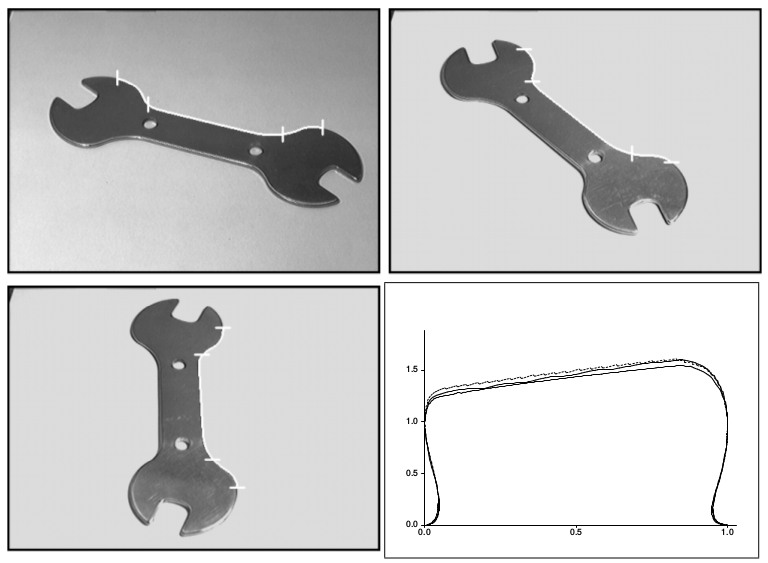
\includegraphics[scale=0.45]{{Images/chap4Invariance}.jpg}}
  \caption{Η αμεταβλητότητα αποτέλεσε πρωταρχικό στόχο των εργασιών ανίχνευσης και αναγνώρισης αντικειμένων. Είναι πρώτιστης σημασίας οι διαφορετικές όψεις του αντικειμένου να έχουν παρόμοια αναπαράσταση στο χώρο των χαρακτηριστικών που χρησιμοποιούνται για την ταυτοποίησή τους. Εδώ για παράδειγμα απεικονίζονται τρεις διαφορετικές όψεις ενός εργαλείου και η συνάρτηση αναπαράστασής τους. Παρατηρούμε την επιθυμητή ομοιότητα μεταξύ των αναπαραστάσεων αυτών. Εικόνα από το \cite{rothwell_1992}.}
  \label{fig:chap4Invariance}
\end{figure}

\par Παράλληλα με τα παραπάνω, δημιουργείται μια άλλη προσέγγιση από τη δεκαετία του '70, η οποία εξελίσσεται με τα χρόνια. Αντί για ταύτιση γεωμετρικών μοντέλων, γίνεται εστίαση στην αναπαράσταση του αντικειμένου ώστε να μπορεί να αναγνωρισθεί ως πρότυπο. Στο \cite{nevatia_1977} γίνεται απόπειρα ανάλυσης αντικειμένων σε απλούστερες δομές, με σκοπό να αυξηθεί η συνθετότητα των αντικειμένων προς αναγνώριση. Στο \cite{marr_1978} επιχειρείται η τρισδιάστατη μοντελοποίηση των αντικειμένων σε δομικά συστατικά. Ωστόσο η δυσκολία αυτής της αναπαράστασης αποτρέπει την καρποφορία των προσεγγίσεων αυτών. Το 1987 το \cite{biederman_1987} επαναφέρει το πρόβλημα με έναν ενδιαφέροντα τρόπο: αναλύει κάθε αντικείμενο σε μονάδες που ονομάζει geons, οι οποίες είναι τρισδιάστατα γεωμετρικά σχήματα με επιππλέον ιδιότητες αμεταβλητότητας σε μετασχηματισμούς. Η θεωρία αυτή έχει ψυχοφυσικό υπόβαθρο \cite{haaf_2003}, \cite{keane_2010} και είναι εύρωστη σε γεωμετρικούς μετασχηματισμούς και αλλαγή οπτικής, δημιουργώντας παράλληλα ένα τεράστιο λεξιλόγιο από συνδυασμούς λίγων μόλις μονάδων. Από την άλλη, η θεωρία δεν συνοδεύτηκε από κάποιο μηχανισμό που να εξάγει τη δομική ανάλυση των αντικειμένων σε μια εικόνα, ενώ αποτυγχάνει να διακρίνει αντικείμενα με παρόμοια δομή σε επίπεδο geons. Οι προσπάθειες δομικής γεωμετρικής αναπαράστασης συνεχίστηκαν, με το \cite{ponce_1989} να εστιάζει σε ανάλυση κυλίνδρων και το \cite{rothwell_1995} σε ανάλυση επιπέδων.

\par Η προσπάθεια αναπαράστασης των αντικειμένων έδωσε το έναυσμα για δύο νέες προσεγγίσεις, τα μοντέλα βασισμένα στην εμφάνιση και τις μεθόδους ανάλυσης χαρακτηριστικών. Το \cite{turk_1991} είναι μια αρκετά πρωτοπόρα εργασία: δημιουργεί ένα μοντέλο προσώπου βασισμένο σε “ιδιοπρόσωπα”, τα οποία είναι ιδιοδιανύσματα πρωταρχικής ανάλυσης σε ένα σύνολο εικόνων προσώπων. Η πρωτοπορία εδώ έγκειται σε πολλά επίπεδα: Διαχωρίζεται η τρισδιάστατη από τη δισδιάστατη προσέγγιση, όπως και η ανίχνευση από την αναγνώριση. Επιπλέον, εισέρχεται η Μηχανική Μάθηση στο προσκήνιο, με την εξαγωγή μαθηματικών χαρακτηριστικών για τη δημιουργία μοντέλου προσώπου αλλά και για τη διάκριση των προσώπων μεταξύ τους, αντί για μεθόδους Όρασης Υπολογιστών αποκλειστικά. Η προσέγγιση αυτή γενικεύεται και αποκτά κάποιον φορμαλισμό στο \cite{murase_1995}, το οποίο απεικονίζει και τις γεωμετρικές πολλαπλότητες που αναπαριστούν ένα αντικείμενο. Η γενική ιδέα είναι η εξαγωγή εμπειρικών μοντέλων με κάποια ικανότητα γενίκευσης. Φορμαλισμό επιχειρεί επίσης να αποδώσει και το \cite{sung_2001}, από τη σκοπιά της εκτίμησης συνάρτησης. Παράλληλα, μια παρόμοια αλλά από διαφορετική σκοπιά προσέγγιση ακολουθείται στο \cite{swain_1991}, όπου αξιοποιούνται ιστογράμματα χρώματος. Οι μέθοδοι μοντέλων εμφάνισης είναι οι πρώτες που θίγουν την απόκριση σε πραγματικό χρόνο. Εν τούτοις, υπάρχουν σαφείς αδυναμίες των χαρακτηριστικών που χρησιμοποιούνται με αποτέλεσμα την ευαισθησία σε απλούς γεωμετρικούς μετασχηματισμούς και επικαλύψεις.

\par Οι μέθοδοι ανάλυσης χαρακτηριστικών είχαν μεγαλύτερη επιτυχία σε επίδοση και ταχύτητα. Ωστόσο η εκπαίδευση γίνεται σε εικόνες που περιέχουν αποκλειστικά το ζητούμενο αντικείμενο και για τον εντοπισμό του αντικειμένου στην εικόνα απαιτείται μια αναζήτηση με κυλιόμενα παράθυρα πάνω στην εικόνα. Γίνονται σημαντικές πρόοδοι σε ανίχνευση αντικειμένων γενικότερα αλλά και πιο ειδικά στην ανίχνευση προσώπου, η οποία ξεκίνησε με το \cite{turk_1991} και συνεχίστηκε στο \cite{belhumeur_1997}. Σταθμό στην ανίχνευση προσώπων αλλά και αντικειμένων γενικότερα αποτελεί αναμφίβολα το \cite{viola_2001}. Η εργασία αυτή εισήγαγε την έννοια των ολοκληρωτικών εικόνων κι επιτάχυνε εξαιρετικά την αναζήτηση πάνω στην εικόνα. Ο ανιχνευτής προσώπου των Viola-Jones είναι γρήγορος και εύρωστος, παρότι απλός, και χρησιμοποιήθηκε για αρκετά χρόνια λόγω αυτών των προτερημάτων του. Ακόμα, εν έτει 2017, το σύστημα αυτό παραμένει ως μια γρήγορη επιλογή για απλά καθήκοντα ανίχνευσης. Τέλος, άξιο αναφοράς αυτή την εποχή είναι και το \cite{schneiderman_2004}, το οποίο εκμεταλλεύεται την πρόοδο της Μηχανικής Μάθησης και επαναφέρει το ζήτημα της αποσύνθεσης του αντικειμένου σε δομικές μονάδες, με αρκετά διαφορετική φύση πλέον.

\begin{figure}
  \centering
  \noindent\makebox[\textwidth]{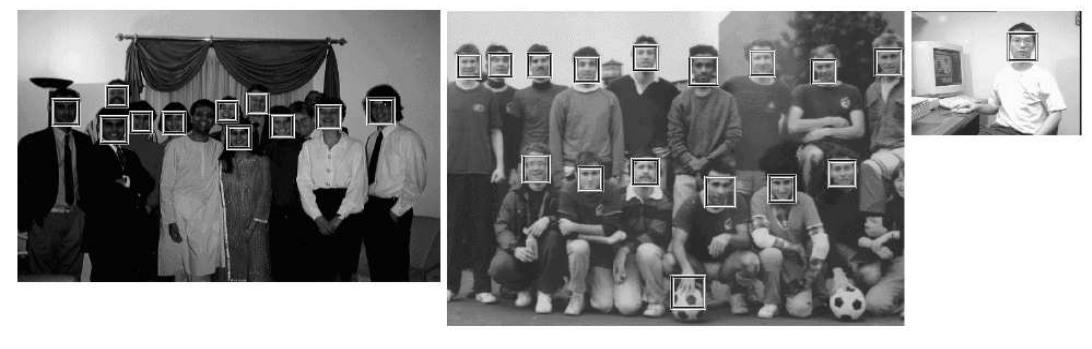
\includegraphics[scale=0.35]{{Images/chap4Viola}.jpg}}
  \caption{Η εργασία των Viola-Jones αποτέλεσε σταθμό στην έρευνα πάνω στην ανίχνευση αντικειμένων χάρη στην απλότητα, ταχύτητα και αποτελεσματικότητά της. Στην εικόνα φαίνονται τα αποτελέσματα της εκτέλεσης του αλγορίθμου ανίχνευσης προσώπου πάνω στις δοθείσες εικόνες. Παρότι η αρχική σχεδίαση έγινε για ανίχνευση προσώπου, η μέθοδος γενικεύεται και δίνει ικανοποιητικά αποτελέσματα για μια ποικιλία αντικειμένων υπό ορισμένες προϋποθέσεις και περιορισμούς στους μετασχηματισμούς που μπορούν να υφίστανται τα ανιχνευόμενα αντικείμενα και απαιτεί μικρό αριθμό θετικών δειγμάτων εκπαίδευσης. Εικόνα από το \cite{viola_2001}.}
  \label{fig:chap4Viola}
\end{figure}

\par Η άνοδος της Μηχανικής Μάθησης και η ταυτόχρονη εξέλιξη του hardware ανοίγουν το δρόμο για μια νέα κατεύθυνση που συνδυάζει εξαγωγή τοπικών χαρακτηριστικών, αμετάβλητες δομές και μοντέλα εμφάνισης. Τα \cite{lowe_1999}, \cite{brown_2002}, \cite{lowe_2004} εισάγουν αναλλοίωτους μετασχηματισμούς και σημεία ενδιαφέροντος, δείχνοντας πώς αυτά μπορούν να χρησιμοποιηθούν στην ανίχνευση αντικειμένων. Στα \cite{mahamud_2003}, \cite{mahamud_2003_optimal} η ανίχνευση γίνεται ορίζοντας μια μετρική απόστασης και λύνοντας ένα πρόβλημα βελτιστοποίησης ως προς αυτή. Το \cite{ferrari_2006} αξιοποιεί τις καμπύλες σαν χαρακτηριστικά των αντικειμένων, το \cite{zhang_2005} εξάγει τοπικά αμετάβλητα χαρακτηριστικά και εστιάζει στο μετασχηματισμό τους με μέθοδο πυρήνα για αποτελεσματικότερη ταξινόμηση και το \cite{fergus_2003} χρησιμοποιεί μια μη επιβλεπόμενη μέθοδο για την εκτίμηση των παραμέτρων των μετασχηματισμών που χρησιμοποιεί. Το \cite{dalal_2005} αποτέλεσε ένα σημαντικό σταθμό εδώ, χρησιμοποιούμενο για χρόνια στην ανίχνευση ανθρώπων. Η εργασία αυτή αναπαριστούσε τοπικά την εικόνα με χαρακτηριστικά HOG και ταξινομούσε με SVM. Τέλος, το \cite{csurka_2004} ήταν από τις πρώτες εργασίες που επέκτειναν το μοντέλο των χαρακτηριστικών σε “σάκο” (bag-of-features), μια ιδέα που είχε ήδη εμφανιστεί πριν αρκετά χρόνια στην κατηγοριοποίηση κειμένου \cite{salton_1983}.

\par Τα τελευταία χρόνια η έρευνα πάνω στην ανίχνευση αντικειμένων έχει γενικευθεί και δεν υπάρχει μαζικός προσανατολισμός. Η εξέλιξη του πεδίου και του υλικού έχουν επιτρέψει την εστίαση πλέον σε πιο δύσκολα εγχειρήματα, όπως ο εντοπισμός παραμορφώσιμων αντικειμένων. Τα \cite{felzenszwalb_2008}, \cite{felzenszwalb_2010} αποτελούν δύο βασικές και πρωτοπόρες εργασίες στην κατεύθυνση αυτή, οι οποίες επαναφέρουν το ζήτημα της διάσπασης ενός σύνθετου αντικειμένου σε μέρη. Το \cite{plagemann_2010} αξιοποιεί δεδομένα βάθους για να πετύχει ανίχνευση μερών του σώματος σε πραγματικό χρόνο, ζήτημα το οποίο πλέον είναι εξέχουσας σημασίας. Προς αυτή την κατεύθυνση γίνονται προσπάθειες όπως του \cite{dean_2013} και τελικά τα συνελικτικά νευρωνικά δίκτυα, μετά την τεράστια επιτυχία τους στην ταξινόμηση \cite{alexnet_2012}, \cite{he_2015}, χρησιμοποιούνται και για ανίχνευση στα \cite{redmon_2015}, \cite{girshick_2015}, με το \cite{huang_2017_state} να πετυχαίνει το πιο πρόσφατο state-of-the-art αποτέλεσμα. Ιδιαίτερη έμφαση έχει δοθεί, λόγω των πολλαπλών εφαρμογών, στην ανίχνευση χεριών τα τελευταία χρόνια \cite{mittal_2011}], \cite{raheja_2011}, \cite{zhu_2014b}, \cite{zhu_2016}, \cite{grzejszczak_2015}, με διαφορετικές προσεγγίσεις είτε για απευθείας εφαρμογές \cite{fratric_2009}, \cite{dawod_2016}, είτε για αλληλεπίδραση με αντικείμενα \cite{kang_2016}, \cite{rosenfeld_ullman_2016}. Τέλος, μια ακόμα αξιόλογη τάση είναι τα μέτρα ύπαρξη αντικειμένου (objectness), τα οποία παράγουν χάρτες που υποδηλώνουν την ύπαρξη ή μη αντικειμένου σε κάθε περιοχή \cite{cheng_2014} και που μπορούν να αξιοποιηθούν για εξαγωγή προσκηνίου σε εικόνες \cite{rother_2004}, \cite{zhu_2014}, \cite{srivatsa_2015}.

\par Κλείνοντας αυτή την ιστορική αναδρομή, θα σχολιάσουμε δύο πράγματα. Το πρώτο αφορά τον ορισμό της ανίχνευσης αντικειμένων που επιζητά την ελάχιστη σε εμβαδόν περιοχή. Η συνθήκη αυτή όταν τηρηθεί αυστηρά καταλήγει στο συγγενικό πρόβλημα της σημασιολογικής κατάτμησης \cite{tighe_2010}, \cite{li_2013}, \cite{zheng_2015},\cite{long_2016}. Το δεύτερο σχόλιο αφορά μια εκτίμηση του επιπέδου στο οποίο βρίσκεται η ανίχνευση αντικειμένων στη σημερινή εποχή. Η ιστορική πορεία δείχνει τεράστια εξέλιξη, ωστόσο ακόμα δεν υπάρχει ενιαίος ανιχνευτής αντικειμένων για κάθε σύνολο δεδομένων και μάλιστα η έρευνα δεν περιστρέφεται γύρω από κοινά σύνολα δεδομένων ώστε να υπάρξει σύγκριση. Επομένως, ένα σύστημα τεχνητής όρασης που θα μπορούσε να πλησιάσει την ανθρώπινη αντίληψη σε φυσικό περιβάλλον είναι ακόμα ένας μακρινός στόχος.


%%%%%%%%%%%%%%%%%%%%%%%%%%%%%%%%%%%%%%%%%%%%%%%% Foreground Detection
\section{Ανίχνευση Προσκηνίου και Παρακολούθηση Αντικειμένων σε Βίντεο}
%%%%%%%%%%%%%%%%%%%%%%%%%% General
\subsection{Γενικά}
Αν δούμε το βίντεο ως ακολουθία εικόνων με σταθερή συχνότητα, είναι φανερό ότι αποδίδουμε μία επιπλέον διάσταση στη συλλογή εικόνων, τον χρόνο. Ωστόσο, μία απεικόνιση του βίντεο ως συνάρτηση τριών διαστάσεων θα έκρυβε τη συσχέτιση των διαδοχικών frames, η οποία επιβάλλει έναν περιορισμό στις μεταβολές των χωρικών συντεταγμένων σε καθορισμένα χρονικά διαστήματα, δηλαδή, αν θεωρήσουμε συνεχή ροή frames, το βίντεο είναι μια περιορισμένη επιφάνεια τριών διαστάσεων όπου οι δύο πρώτες συντεταγμένες είναι συναρτήσεις της τρίτης. Είναι και διαισθητικά αλλά και μαθηματικά φανερό ότι μπορούμε επομένως να μιλάμε για δύο χρονικά μεταβαλλόμενες χωρικές συναρτήσεις, εισάγοντας την έννοια της κίνησης και της ταχύτητας. Η ανίχνευση προσκηνίου και η παρακολούθηση αντικειμένων μόνο τότε αποκτούν υπόσταση. Εύκολα κανείς θα αντιλαμβανόταν ότι η παρακολούθηση αντικειμένων σε βίντεο, εφόσον έχει αίσθηση της έννοιας του αντικειμένου, είναι ο προσδιορισμός της θέσης του αντικειμένου σε κάθε χρονική στιγμή. Η παρακολούθηση είναι δηλαδή η γενίκευση της ανίχνευσης σε ακολουθία συσχετιζόμενων εικόνων. Για το ποιο είναι το προσκήνιο σε μια εικόνα ή βίντεο ωστόσο δεν υπάρχει μαθηματικός ορισμός, πρόκειται για ένα πρόβλημα μη καλώς ορισμένο. Στην περίπτωση των ακίνητων εικόνων είδαμε ότι τα τελευταία χρόνια νέοι ορισμοί δίνονται και προσπάθειες γίνονται για το λεγόμενο μέτρο “objectness”, την ύπαρξη αντικειμένου του προσκηνίου στην κάθε θέση. Στα βίντεο συνήθως ορίζουμε ως προσκήνιο τα κινούμενα αντικείμενα, δηλαδή τις θέσεις μεταβολών μεταξύ διαδοχικών frames. Το δυικό πρόβλημα του προσκηνίου είναι η εξαγωγή μοντέλου παρασκηνίου. Τα δύο προβλήματα είναι πρακτικά ισοδύναμα κι οι όροι χρησιμοποιούνται εναλλακτικά ανάλογα με το σκοπό δράσης.

\begin{figure}
  \centering
  \noindent\makebox[\textwidth]{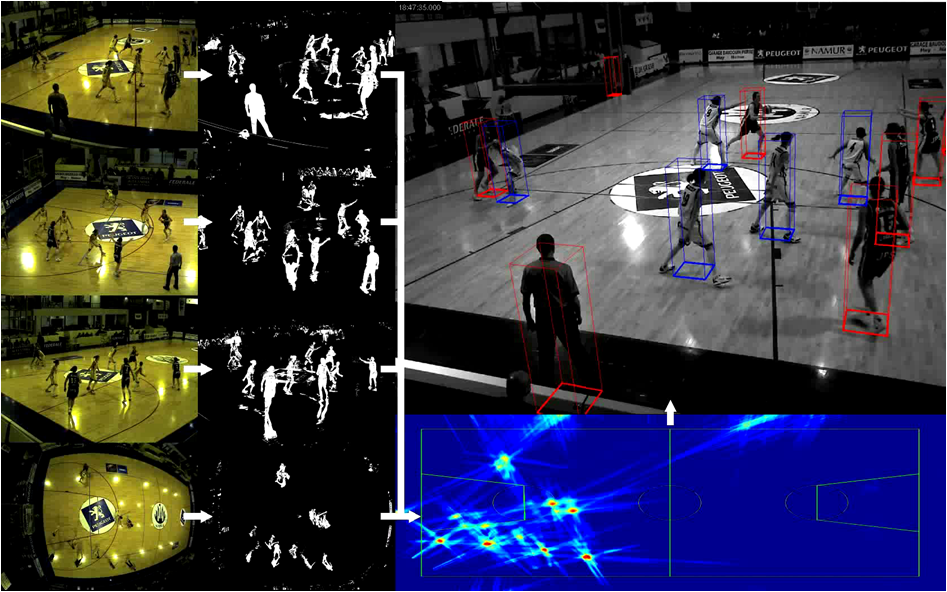
\includegraphics[scale=0.7]{{Images/chap4Foregd}.png}}
  \caption{Ζήτημα της ανίχνευσης προσκηνίου είναι η εύρεση όχι μόνο των κινούμενων αντικειμένων αλλά και των κινήσεων ενδιαφέροντος. Παρότι ο ορισμός αυτός δεν είναι σαφής, διαισθητικά ζητάμε την κίνηση που αφορά την απεικονιζόμενη δράση στην οποία και εστιάζουμε και όχι πιθανές άλλες δράσεις που μπορεί να συμβαίνουν στο περιβάλλον, κάτι που ονομάζουμε παρασκήνιο. Στο εικονιζόμενο παράδειγμα, προσκήνιο αποτελούν οι αθλήτριες και η μπάλα, αλλά όχι κάποια κίνηση που μπορεί να πραγματοποιείται στην εξέδρα. Εικόνα από το \cite{delannay_2009}.}
  \label{fig:chap4Foregd}
\end{figure}

\par Είναι φανερό ότι η παρακολούθηση αντικειμένων αλλά κυρίως η ανίχνευση προσκηνίου, που δεν είναι καλώς ορισμένο πρόβλημα, παρουσιάζουν ποικίλες προκλήσεις. Οι αλλαγές στον φωτισμό, η σκίαση, ο θόρυβος και η κίνηση της κάμερας είναι ίσως αυτές που έχουν μοντελοποιηθεί αποτελεσματικότερα. Σημαντικές δυσκολίες επιβάλλει το ίδιο το παρασκήνιο. Συχνά, υπάρχουν επικαλύψεις του αντικειμένου κίνησης με αντικείμενα του παρασκηνίου ή το παρασκήνιο παρέχει “καμουφλάζ” σε αντικείμενα του προσκηνίου. Ακόμα χειρότερα είναι τα πράγματα όταν έχουμε να κάνουμε με δυναμικό υπόβαθρο: αν θυμηθούμε τον ορισμό που επιχειρήσαμε να δώσουμε για το προσκήνιο, βλέπουμε ότι κάθε κίνηση, η οποία θα προκαλεί αλλαγή μεταξύ δύο διαδοχικών frames, πρέπει να ερμηνεύεται ως προσκήνιο. Αυτό όμως δεν ισχύει, καθώς αντικείμενα του παρασκηνίου μπορεί να μεταβάλλουν την εμφάνισή τους, για παράδειγμα μια ανοιχτή τηλεόραση ή ένα αυτοκίνητο που διέρχεται αρκετά μέτρα πίσω από αυτό που καταγράφει η κάμερα, ή ακόμα και οι καιρικές συνθήκες να δυσχεραίνουν τη διάκριση του αντικειμένου \cite{prasad_2016}. Από τα τελευταία παραδείγματα γίνεται εμφανές το πόσο εύθραυστος είναι ο ορισμός που δώσαμε για το προσκήνιο. Οι άνθρωποι τείνουν να θεωρούν προσκήνιο αυτή τη δράση οποία εξελίσσεται μπροστά τους κι έχει “ενδιαφέρον” για το δράστη και το σκοπό δράσης. Ακόμα κι αν ο δράστης σταματήσει να κινείται, οπότε αποτελεί παρασκήνιο με τον αρχικό ορισμό, μπορεί να δρα, άρα να αποτελεί προσκήνιο. Τέλος, υπάρχουν και αντικειμενικές δυσκολίες που πρέπει να ληφθούν υπόψιν, όπως η μοντελοποίηση της κίνησης ενός αντικειμένου με άγνωστη συνάρτηση ταχύτητας (συμπεριλαμβανομένου και γωνιακής ταχύτητας) και η ανεπάρκεια δεδομένων για εξαγωγή μοντέλου περιβάλλοντος.

\par Όσο δύσκολο κι αν είναι το πρόβλημα της ανίχνευσης προσκηνίου και της παρακολούθησης αντικειμένων, τόσο χρήσιμη είναι η εφαρμογή των αποτελεσμάτων του σε πολλές πτυχές της καθημερινότητας. Συστήματα επίβλεψης, ανιχνευτές κίνησης, προγράμματα αλληλεπίδρασης ανθρώπου-μηχανής, εξαγωγή περιεχομένου από βίντεο και αναγνώριση χειρονομιών σε πραγματικό χρόνο είναι μερικές από τις πολυάριθμες εφαρμογές των ανιχνευτών κίνησης και προσκηνίου. Πιο συγκεκριμένα, τα αυτόματα αυτοκίνητα του μέλλοντος πρέπει να διαθέτουν μηχανισμούς εντοπισμού πεζών ή επικίνδυνων αντικειμένων σε πραγματικό χρόνο \cite{dollar_2010}, ενώ συστήματα υποβοήθησης ηλικιωμένων πρέπει να ανιχνεύουν επιτυχώς τις κινήσεις που τα αφορούν \cite{rodomagoulakis_2016}. Στη σφαίρα αυτή, πολλές έρευνες έχουν γίνει και γίνονται πάνω στην παρακολούθηση αντικειμένων και στην ανίχνευση προσκηνίου.

%%%%%%%%%%%%%%%%%%%%%%%%%%%% History
\subsection{Ιστορικά Στοιχεία}
Η πρώτη προσέγγιση παρακολούθησης που εφαρμόστηκε ήταν με τη χρήση σημείων. Συγκεκριμένα., το αντικείμενο αναπαρίσταται ως ένα σύνολο σημείων και παρακολουθείται κάθε σημείο ξεχωριστά. Στα μέσα της δεκαετίας του '80 κυριαρχούν οι στατιστικές μέθοδοι παρακολούθησης σημείων και πρώτο το \cite{broida_1986} κάνει χρήση του φίλτρου Kalman \cite{kalman_1960} για την παρακολούθηση σημείων σε θορυβώδεις εικόνες. Στο \cite{beymer_1999} συνεχίζεται η ίδια προσέγγιση, ενώ το \cite{rosales_1999} επεκτείνει τη χρήση του φίλτρου για να εκτιμήσει τρισδιάστατες τροχιές από δισδιάστατη κίνηση. Σε παρόμοιο πλαίσιο, τα \cite{chang_1991} και \cite{rasmussen_2001} χρησιμοποιούν τον πιο ευσταθή αλγόριθμο JPDAF, ενώ τα \cite{streit_1994}, \cite{cox_1996}, \cite{cham_1999} κάνουν χρήση πιθανοτικών ή υπολογιστικά αποδοτικότερων παραλλαγών του πιο εύρωστου αλγορίθμου MHT \cite{reid_1979}. Συγγενική αλλά πιο προχωρημένη, η προσέγγιση του \cite{hue_2002} χρησιμοποιεί στατιστικές μεθόδους και φίλτρα σωματιδίων. Παράλληλα με τις στατιστικές αναπτύσσονται και ντετερμινιστικές μέθοδοι παρακολούθησης, με τα \cite{sethi_1987}, \cite{salari_1990} και \cite{rangarajan_1991} να κάνουν την αρχή και τα \cite{intille_1997}, \cite{veenman_2001}, \cite{shafique_2003} να βελτιώνουν τις προσεγγίσεις αυτές. Γενικά, η αναπαράσταση των αντικειμένων ως σύνολα σημείων την εποχή εκείνη είχε περιορισμένη επιτυχία καθώς βασίζονταν πάνω σε αυστηρές υποθέσεις για την κατανομή θορύβου και τη μορφή των αντικειμένων οι οποίες συχνά δε μοντελοποιούν μια γενικευμένη πραγματικότητα.

\par Μια διαφορετική προσέγγιση του προβλήματος της οπτικής παρακολούθησης αντικειμένων ήταν αυτή της λεγόμενης “παρακολούθησης πυρήνα”, όπου το αντικείμενο αναπαρίσταται από ένα γεωμετρικό σχήμα ή μια συμπαγή περιοχή του χώρου και μελετάται η κίνηση αυτής της περιοχής, συνήθως με προσεγγίσεις κλασσικών γεωμετρικών μετασχηματισμών ή υπολογισμό οπτικής ροής. Δύο σχολές διαμορφώθηκαν εδώ, ανάλογα με την αναπαράσταση του αντικειμένου. Η πρώτη δίνει έμφαση στον εντοπισμό του αντικειμένου και στην παρακολούθηση κίνησης ανανεώνοντας τον εντοπισμό, ενώ η αναπαράσταση γίνεται με πρότυπα \cite{birchfield_1998} ή μοντέλα μίξης \cite{jepson_2003}, ιστογράμματα χρώματος \cite{fieguth_1997} και άλλες σχετικες μεθόδους \cite{liu_2002}. Ιδιαίτερης αναφοράς χρίζουν τα \cite{lucas_1981}, \cite{shi_1994} και \cite{comaniciu_2002}, \cite{comaniciu_2003} τα οποία αποτελούν ακόμα και σήμερα ρεαλιστικές και επίκαιρες εναλλακτικές. Ξεχωριστές για την πρώτη σχολή καθώς πετυχαίνουν παρακολούθηση πολλών αντικειμένων ταυτόχρονα είναι οι εργασίες των \cite{isard_2001}, που μοντελοποιεί παρασκήνιο και προσκήνιο με μοντέλα μίξης γκαουσιανών, και \cite{tao_2002} που απεικονίζει τα frames σαν ένα σύνολο επιπέδων (παρασκήνιο και αντικείμενα) ορίζοντας ως παραμέτρους το σχήμα, την κίνηση και την εμφάνιση. Η δεύτερη σχολή, αντί να παρακολουθεί στη διάρκεια του βίντεο ένα αντικείμενο εξάγοντας το μοντέλο του από πιθανοτικές μεθόδους, πρώτα δημιουργεί ένα μοντέλο συνδυάζοντας εικόνες από διαφορετικές όψεις έτσι ώστε να αποκτά ευρωστία σε γεωμετρικούς μετασχηματισμούς. Το πλεονέκτημα αυτών των μεθόδων είναι η γνώση ότι παρακολουθείται το ίδιο αντικείμενο κι όχι όποιο αντικείμενο κινείται. Το \cite{black_1998} χρησιμοποιεί Ανάλυση Πρωταρχικών Συνιστωσών (PCA) για να αναπαραστήσει και να ανακατασκευάσει το αντικείμενο, μεταφέροντας τη σύγκριση προτύπων (εναλλακτική του ταιριάσματος) στο χώρο των ιδιοδιανυσμάτων. Σε παρόμοια κατεύθυνση, το \cite{avidan_2001} χρησιμοποιεί Μηχανές Διανυσματικής Υποστήριξης (SVM) για να εκπαιδεύσει τον παρακολουθητή χρησιμοποιώντας ως αρνητικά δείγματα περιοχές του παρασκηνίου που μοιάζουν με το αντικείμενο.

\par Οι προσεγγίσεις παρακολούθησης πυρήνα βασίζονται στην υπόθεση της δυνατότητας αναπαράστασης των αντικειμένων με απλά γεωμετρικά σχήματα τα οποία παραμένουν σχετικά αναλλοίωτα στο χρόνο. Η υπόθεση αυτή παρέχει ταχύτητα στο σύστημα αλλά δεν είναι πάντα εύλογη, συν ότι το παρασκήνιο μπορεί να απεικονίζεται με παρόμοια γεωμετρικά σχήματα. Η μεταβλητότητα, η παραμορφωσιμότητα και η συνθετότητα των αντικειμένων ήταν η αιτία αναζήτησης πιο εκλεπτυσμένων μεθόδων αναπαράστασης και παρακολούθησης, όπως η “παρακολούθηση σιλουέτας”. Μια απλή αλλά αδύναμη προσέγγιση είναι το ταίριασμα σχήματος με την υπόθεση ότι μεταξύ διαδοχικών frames μπορεί να πραγματοποιηθεί μόνο μετάθεση του αντικειμένου και με χρήση του μετασχηματισμού Hausdorff \cite{huttenlocher_1993}, \cite{li_2001}. Μια εναλλακτική στο ταίριασμα σχήματος είναι η μοντελοποίηση του αντικειμένου με ιστογράμματα χρώματος και ακμές \cite{kang_2004}, ενώ το \cite{haritaoglu_2000} χρησιμοποιεί πληροφορία από τις ακμές εντός της περιοχής της σιλουέτας για να εντοπίσει το αντικείμενο. Τέλος, το \cite{sato_2004} χειρίζεται διαφορετικά το πρόβλημα, εφαρμόζοντας τον μετασχηματισμό Hough στο χώρο των ταχυτήτων.

\begin{figure}
  \centering
  \noindent\makebox[\textwidth]{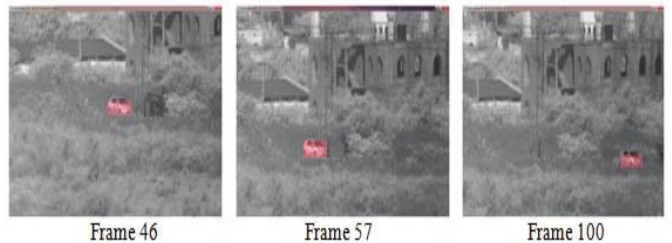
\includegraphics[scale=0.6]{{Images/chap4TrackEx}.jpg}}
  \caption{Παρακολούθηση κινούμενου αυτοκινήτου σε πραγματικό χρόνο με τη βοήθεια Κάρτας Γραφικών Υπολογιστή (GPU). Παρατηρούμε ότι η κάμερα κινείται και ως εκ τούτου η σχετική θέση κάμερας και περιβάλλοντος μεταβάλλεται διαρκώς. Εν τούτοις το σύστημα κατορθώνει να απομονώνει το αντικείμενο ενδιαφέροντος και να κατατάσσει την υπόλοιπη εικόνα ως παρασκήνιο. Οι κάρτες γραφικών συνέβαλλαν δραστικά στην αύξηση της ταχύτητας υπολογισμών για τις απαιτητικές εφαρμογές της σημεριωής εποχής. Εικόνα από το \cite{mistree_2015}.}
  \label{fig:chap4TrackEx}
\end{figure}

\par Η παρακολούθηση σιλουέτας εκφράστηκε ποιοτικότερα από τις μεθόδους καμπυλών. Οι μέθοδοι αυτές παρακολουθούν την εξέλιξη καμπυλών σε διαδοχικά frames και μπορούν να διακριθούν σε δύο βασικές κατευθύνσεις. Η πρώτη, αναπαριστά το σχήμα και την κίνηση της καμπύλης ως εσωτερικές μεταβλητές στο χώρο καταστάσεων. Η ιδέα ξεκινά ήδη από το 1992 με το \cite{terzopoulos_1992} και αναπτύσσεται στα \cite{isard_1998}, \cite{peterfreund_1999}. Το \cite{maccormick_2000} επεκτείνει το μοντέλο ώστε να διαχειρίζεται επικαλύψεις και να παρακολουθεί πληθώρα αντικειμένων, ενώ το \cite{Chen_2001} μοντελοποιεί την εξέλιξη της καμπύλης με Κρυφά Μαρκοβιανά Μοντέλα (HMM). Η δεύτερη κατεύθυνση στράφηκε προς την ελαχιστοποίηση του συναρτησοειδούς της ενέργειας καμπύλης. Η ενέργεια της καμπύλης οριζόταν σε όρους χρονικής πληροφορίας με τη μορφή είτε χρονικών παραγώγων (οπτική ροή) \cite{bertalmio_2000}, \cite{mansouri_2002}, \cite{cremers_2003}, είτε με στατιστικά εμφάνισης παραγόμενα από τις περιοχές αντικειμένων και τις περιοχές παρασκηνίου \cite{yilmaz_2004}, \cite{ronfard_1994}. Στην πρώτη περίπτωση έχουμε χρήση του Λογισμού Μεταβολών ως βασικό εργαλείο, ενώ στη δεύτερη χρησιμοποιούνται ευριστικές μέθοδοι. Ωστόσο, παρά τη δύναμη και την ευελιξία τους, οι μέθοδοι παρακολούθησης σιλουέτας πάσχουν στην περίπτωση ανάμιξης ή διαχωρισμού των αντικειμένων, για παράδειγμα όταν ένας άνθρωπος αφήνει ή λαμβάνει ένα αντικείμενο του περιβάλλοντος, αλλά και (λιγότερο) στην περίπτωση ισχυρών επικαλύψεων των αντικειμένων. Μια σύνοψη και σύγκριση των παραπάνω αλγορίθμων γίνεται στο \cite{yilmaz_2006}, ενώ μια πιο πρόσφατη προσέγγιση γίνεται στο \cite{lakshmeeswari_2016}.

\par Στα τελευταία χρόνια η έρευνα έχει γενικευθεί και πλέον η απαιτητικότητα των εφαρμογών έχει ωθήσει προς νέες κατευθύνσεις την παρακολούθηση αντικειμένων. Μεγάλη έμφαση δίνεται στην απόκριση σε πραγματικό χρόνο \cite{lei_2011}, \cite{kodjo_2012}, απαίτηση που είχε ήδη εμφανιστεί και παλιότερα \cite{comaniciu_2000}, \cite{kim_2008}. Η εξέλιξη αυτή υποβοηθείται από τις σύγχρονες καινοτομίες σε hardware και software \cite{mistree_2015}, \cite{lyu_2016}, \cite{yasukawa_2016}. νέες μέθοδοι γεννιούνται \cite{mehta_2014}, \cite{misra_2015}, ενώ ταυτόχρονα οι παλιότερες συνεχίζουν να αναπτύσσονται \cite{deori_2014}. Όπως και στην ανίχνευση αντικειμένων, έτσι και στην παρακολούθηση, έχει δοθεί σήμερα μια ξεχωριστή ροή μελέτης για την περίπτωση των ανθρώπινων χεριών \cite{chen_2014}, \cite{sridhar_2015}, \cite{sharp_2015}, καθώς είναι το κύριο όργανο δράσης των ανθρώπων ενώ παράλληλα παρουσιάζει τεράστια ποικιλομορφία και κατ'επέκταση μοντελοποιείται δύσκολα. Για διαφορετικές εφαρμογές χρησιμοποιούνται και διαφορετικές οπτικές κάμερας, οπότε έχουμε ειδικά συστήματα σχεδιασμένα για κάμερες βάθους \cite{sridhar_2016} και για “εγωκεντρικά” βίντεο \cite{li_2013_pixel}, \cite{zhu_2016}.

\par Η ανίχνευση προσκηνίου, ως συγγενική της παρακολούθησης εργασία αναπτύχθηκε παράλληλα και συχνά χρησιμοποιήθηκε για την παρακολούθηση \cite{isard_2001}. Κύρια ιδέα είναι η χρήση γκαουσιανών μοντέλων μίξης για την περιγραφή του προσκηνίου και του παρασκηνίου με την αρχή να γίνεται το 1999 \cite{stauffer_1999} και την ιδέα να βελτιώνεται λίγο αργότερα \cite{kaewtrakulpong_2002}. Οι ιδέες αυτές παρέμειναν στο επίκεντρο της έρευνας για τα επόμενα χρόνια \cite{wang_2005} και το \cite{bouwmans_2008} παρέχει μια σύνοψη μεγάλου αριθμού αυτών. Η χρήση μοντέλων μίξης παραμένει σαν μια δυνατή εναλλακτική μέχρι σήμερα, ωστόσο τα τελευταία χρόνια έχουν αναπτυχθεί και άλλες μέθοδοι. Τα \cite{jenifa_2012}, \cite{bouwmans_2014} προσεγγίζουν το ζήτημα από τη δυική του μορφή (εξαγωγή παρασκηνίου). Καθώς η ανάγκη για απόκριση πραγματικού χρόνου γίνεται πιο πιεστική, νέες εργασίες ασχολούνται με την ανίχνευση προσκηνίου με χρήση αλγορίθμων αυτο-οργανούμενης εξαγωγής παρασκηνίου (SOBS) \cite{maddalena_2012}, προσαρμοστικής κατάτμησης σε επίπεδο πίξελ (PBAS) \cite{hofmann_2012} και εξαγωγής οπτικού παρασκηνίου (ViBe) \cite{barnich_2009}. Μάλιστα στο \cite{kryjak_2013} γίνεται μια υλοποίηση του ViBe σε FPGA. Τέλος, τα νευρωνικά δίκτυα χρησιμοποιούνται επίσης στην ανίχνευση προσκηνίου \cite{ruchanurucks_2006} και μάλιστα πλέον έχουν χρησιμοποιηθεί και βαθιά συνελικτικά νευρωνικά δίκτυα \cite{braham_2016}, \cite{babaee_2017}.


%%%%%%%%%%%%%%%%%%%%%%%%%%%%%%%%%%%%%%%%%%%%%%% Theory
\section{Θεωρητικό Υπόβαθρο}
%%%%%%%%%%%%%%%%%%%%%%% Template Matching
\subsection{Ταίριασμα Προτύπων (Template Matching)}
Η μέθοδος ταιριάσματος προτύπων (template mathing) είναι μία απλή και σχετικά γρήγορη αλλά περιορισμένης αποτελεσματικότητας μέθοδος εντοπισμού αντικειμένων σε εικόνες. Συνοπτικά, έχοντας στη διάθεσή της μια αναπαράσταση του αντικειμένου, μία δηλαδή εικόνα του, αναζητά την περιοχή της εικόνας για την οποία μεγιστοποιείται μια συνάρτηση ταιριάσματος μεταξύ της περιοχής αυτής και του προτύπου για το αντικείμενο. Διαισθητικά, πρόκειται για έναν ανιχνευτή αντικειμένων εκπαιδευμένο με μόνο ένα δείγμα για το αντικείμενο που ζητάμε. Είναι φανερό ότι ένας τέτοιος ανιχνευτής, ή ένα οποιοδήποτε σύστημα με δυνατότητα μάθησης, θα παρουσίαζε υψηλή υπερπροσαρμογή στο πρότυπο: τίποτα δεν αποτελεί δείγμα αυτής της κατηγορίας αντικειμένου εκτός αν ταιριάζει ακριβώς με το πρότυπο. Θα δούμε τα πλεονεκτήματα και μειονεκτήματα ενός τέτοιου ανιχνευτή αντικειμένων αφού εξετάσουμε την υλοποίησή του.

\begin{figure}
  \centering
  \noindent\makebox[\textwidth]{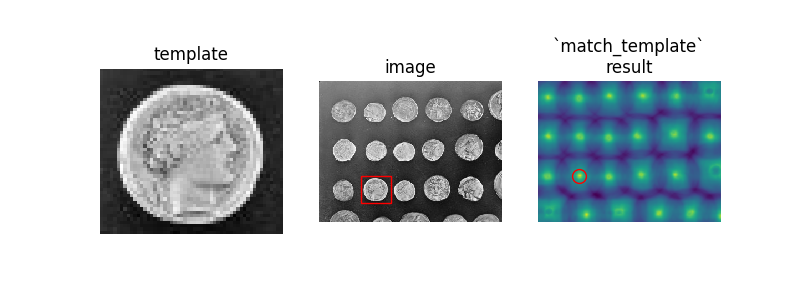
\includegraphics[scale=0.7]{{Images/chap4Template}.png}}
  \caption{Η λογική της μεθόδου Ταιριάσματος Προτύπων: Δοθεντος ενός προτύπου, αναζητούμε τη βέλτιστη τοποθέτησή του στην εικόνα έτσι ώστε να μεγιστοποιείται μια συνάρτηση ομοιότητας μεταξύ προτύπου και τμηματος εικόνας. Η συνάρτηση ομοιότητας μπορεί να επιλεχθεί κατάλληλα σύμφωνα με το πρόβλημα και τις απαιτήσεις του σχεδιαστή. Συχνά, χρησιμοποιείται κατώφλι στη συνάρτηση ομοιότητας και τιμές μικρότερες αυτού σημαίνουν μη ταίριασμα και απουσία του προτύπου από την εικόνα.}
  \label{fig:chap4Template}
\end{figure}

\par Τρεις απλές υλοποιήσεις ταιριάσματος προτύπων είναι οι μέθοδοι Φίλτρου Μηδενικής Μέσης Τιμής (Zero-Mean Filter), Αθροίσματος Τετραγωνικών Διαφορών (SSD: Sum of Squared Differences) και Κανονικοποιημένης Ετεροσυσχέτισης. Στην πρώτη μέθοδο, φιλτράρουμε την εικόνα με το πρότυπο, έχοντας αφαιρέσει από αυτό τη μέση τιμή του και αναζητούμε μέγιστα της εξόδου. Στη δεύτερη, υπολογίζουμε για κάθε περιοχή της εικόνας το άθροισμα των τετραγώνων των διαφορών μεταξύ των pixels της εικόνας και των pixels του προτύπου, αναζητώντας ελάχιστα της εξόδου, ή ισοδύναμα, μέγιστα της αντίθετης συνάρτησης της εξόδου. Τέλος, η τρίτη μέθοδος συνδυάζει τις δύο προηγούμενες εισάγοντας την κανονικοποιημένη ετεροσυσχέτιση μεταξύ προτύπου και τμήματος εικόνας. Η μέθοδος αυτή είναι η πιο αργή αλλά και η πιο αποτελεσματική, καθώς πετυχαίνει αμεταβλητότητα τοπικά στη μέση ένταση της εικόνας και στην αντίθεση. Αμέσως γρηγορότερη είναι η μέθοδος SSD, η οποία όμως είναι ευαίσθητη στη μεταβολή της έντασης της εικόνας. Τέλος, ακόμα πιο γρήγορη είναι η πρώτη μέθοδος, αλλά ταυτόχρονα είναι και η λιγότερη εύρωστη.

\par Θα περιγράψουμε με λίγη περισσότερη λεπτομέρεια τώρα τη μέθοδο SSD για ταίριασμα προτύπων. Έστω $f[x,y]$ μια εικόνα και $g[x,y]$ ένα πρότυπο. Υπολογίζουμε το άθροισμα των τετραγωνικών διαφορών σε κάθε περιοχή που προκύπτει από την ολίσθηση του προτύπου πάνω στην εικόνα ως εξής:

\begin{equation}\label{eq:SSD}
    h[x,y]=\sum_{(k,l)} (g[k,l]-f[k+x,l+y])^{2}
\end{equation}

Λαμβάνουμε ως έξοδο την $1-h[x,y]$, η οποία θα είναι μέγιστη, κοντά στην τιμή 1, όταν το άθροισμα στην έκφραση της $h$ λαμβάνει χαμηλές τιμές, οπότε πρότυπο και εικόνα παρουσιάζουν υψηλή ταύτιση. Εφαρμόζουμε ένα κατώφλι στην έξοδο της $1-h$ έτσι ώστε να κρατήσουμε μόνο τις περιοχές υψηλής ταύτισης ως πιθανές περιοχές του αντικειμένου. Είναι φανερό από τον ορισμό της $h$, ότι απόλυτη ταύτιση συμβαίνει μόνο όταν $h=0$, οπότε πρότυπο και εικόνα ταιριάζουν σχηματικά και χρωματικά. Ο ορισμός της $h$, αφήνει τη μέθοδο ευάλωτη σε διακυμάνσεις έντασης και φωτισμού. Πράγματι, ένα οποιοδήποτε scaling της εικόνας χρωματικά ($f \to \alpha*f$, $\alpha$ πραγματικός αριθμός) θα μας δώσει σαν έξοδο την ενέργεια του τμήματος της εικόνας που εξετάζουμε επί έναν πολλαπλασιαστικό παράγοντα $(1-\alpha)^{2}$. Δηλαδή, όσο μεγαλύτερη η μεταβολή της φωτεινότητας (υποθέτοντας ομοιόμορφη μεταβολή τοπικά) και άρα όσο πιο μεγάλη η απόσταση του α από τη μονάδα, τόσο μεγαλύτερη η αποτυχία ταύτισης. Θα δούμε τώρα πώς η μέθοδος αυτή μπορεί να υλοποιηθεί αποδοτικά, έτσι ώστε να αξιοποιηθεί η ταχύτητά της.

\par Ξεκινάμε από τη μορφή της $h$ που δίνεται στην εξίσωση \eqref{eq:SSD}. Εύκολα διαπιστώνουμε ότι

\begin{equation}\label{eq:SSD2}
    h[x,y]=\sum_{(k,l)} f^{2}[k+x,l+y] + \sum_{(k,l)} g^{2}[k,l] -s\sum_{(k,l)} (g[k,l]f[k+x,l+y])
\end{equation}

Τώρα είναι φανερό ότι ο πρώτος όρος είναι σταθερός ως προς $x$ και $y$ και αρκεί να υπολογιστεί μία φορά. Για τον δεύτερο όρο, αντί να αθροίζουμε κάθε φορά όλα τα pixels, μπορούμε να χρησιμοποιήσουμε τη μέθοδο των ολοκληρωτικών εικόνων \cite{viola_2001}, δηλαδή να υπολογίσουμε σε κάθε θέση το συσσωρευτικό άθροισμα όλων των τιμών των pixels με τιμές $x$ και $y$ μικρότερες είτε ίσες με αυτές της τρέχουσας θέσης. Από εκεί και πέρα, το πρόβλημα υπολογισμού ενός αθροίσματος pixels σε μια συγκεκριμένη περιοχή εικόνας είναι της κλάσης $O(1)$. Τέλος, ο τρίτος όρος του αθροίσματος περιέχει ένα άθροισμα το οποίο αποτελεί τη συσχέτιση $f$ και $g$. Για τον αποδοτικό υπολογισμό της συσχέτισης, αφού εφαρμόσουμε κατάλληλο zero-padding στις $f$ και $g$, περιστρέφουμε την $g$ κατά 90 μοίρες και υπολογίζουμε το εσωτερικό γινόμενο των μετασχηματισμών Fourier της περιστραμμένης $g$ και της $f$. Η συσχέτιση είναι ίση με το πραγματικό μέρος του αντίστροφου μετασχηματισμού Fourier αυτού του εσωτερικού γινομένου. Οπότε συνολικά, η ποσότητα SSD μπορεί να υπολογιστεί γρήγορα και αποδοτικά.

\par Έχοντας δει και λεπτομέρειες υλοποίησης, είμαστε σε θέση να διακρίνουμε πλέον τα υπέρ και τα κατά της χρήσης μιας τέτοιας μεθόδου για ανίχνευση αντικειμένων. Από άποψη ταχύτητας, είδαμε ότι με κατάλληλη υλοποίηση ένας αλγόριθμος ταιριάσματος προτύπων μπορεί να γίνει εξαιρετικά γρήγορος. Ας σχολιάσουμε κυρίως όμως το φλέγον ζήτημα της αποτελεσματικότητας αλλά και της δυνατότητας γενίκευσης. Είδαμε ότι για τον έλεγχο ταιριάσματος εφαρμόζεται κατώφλι το οποίο εύκολα απορρίπτει ένα τμήμα εικόνας μόνο και μόνο λόγω διαφορετικού φωτισμού. Ωστόσο για μικρές διακυμάνσεις φωτισμού είναι δυνατό να επιτευχθεί ταίριασμα. Το πρότυπο αποτελεί τη μοναδική εικόνα εκπαίδευσης και άρα τη μοναδική αναπαράσταση του αντικειμένου. Από την μία αυτό αφαιρεί τη διαδικασία εκπαίδευσης, από την άλλη όμως στερεί οποιαδήποτε δυνατότητα γενίκευσης. Ακόμα χειρότερα, η εικόνα προτύπου πιθανότατα περιλαμβάνει και μικρό τμήμα παρασκηνίου, καθιστώντας την ανίχνευση ευάλωτη ακόμα και σε μεταθέσεις του ίδιου αντικειμένου μπροστά από διαφορετικό παρασκήνιο. Παρόλα αυτά, η μέθοδος παραμένει χρήσιμη στην ανίχνευση αντικειμένων με χαμηλή οπτική μεταβλητότητα και κίνηση σε βίντεο. Υπάρχουν περιπτώσεις που σε ένα βίντεο μας αρκεί να εντοπίζουμε σταθερά πρότυπα αντικειμένων τα οποία μένουν πρακτικά αναλλοίωτα για μεγάλο χρονικό διάστημα. Σε αυτές τις περιπτώσεις είναι που το ταίριασμα προτύπων μπορεί να δώσει εξαιρετικά και γρήγορα αποτελέσματα.

%%%%%%%%%%%%%%%%%%%%%%%%% GMM Foreground
\subsection{Εξαγωγή Προσκηνίου με Μοντέλα Μίξης Γκαουσιανών (GMM)}
Μια δημοφιλής μέθοδος εξαγωγής προσκηνίου είναι η χρήση Μοντέλων Μίξης Γκαουσιανών. Η μέθοδος εισήχθη στο \cite{stauffer_1999} και βελτιώθηκε στο \cite{kaewtrakulpong_2002} ώστε να μοντελοποιεί τη μεταβολή στη σκίαση και να μην τη συνυπολογίζει στην κίνηση. Η βασική ιδέα είναι η μοντελοποίηση κάθε πίξελ ως ένα άθροισμα γκαουσιανών με βάρη (μίξη). Επομένως, η πιθανότητα ένα συγκεκριμένο πίξελ να έχει τιμή $x_N$ τη χρονική στιγμή $N$ εκφράζεται από τη σχέση:

\begin{equation}\label{eq:GMM}
    p(x_N)=\sum_{k=1}^{K} w_k \eta(x_N; \theta_{k})
\end{equation}

με την παράμετρο $w_k$ να εκφράζει το βάρος της $k$-οστής Γκαουσιανής $\eta(x,\theta_{k})$, με τη συνάρτηση αυτή να δίνεται από τη σχέση

\begin{equation}\label{eq:Gaussian}
    \eta(x_N; \theta_{k})=\eta(x_N; \mu_{k}, \Sigma_{k})=\frac{1}{2\pi^{\frac{D}{2}} | \Sigma_{k} |^{\frac{1}{2}}}e^{-\frac{1}{2}(x-\mu_k)^{T}\Sigma_{k}(x-\mu_k)}
\end{equation}

όπου $\mu_{k}$ είναι η μέση τιμή και $\Sigma_{k}$ η συνδιακύμανση της $k$-οστής συνιστώσας.

\par Η μέθοδος εκκινεί με την αρχική εκτίμηση του μοντέλου μίξης μέσω συναρτήσεων ανανέωσης προσδοκώμενων επαρκών στατιστικών. Μετά τα $L$ πρώτα δείγματα χρησιμοποιείται η παραλλαγή των $L$-πρόσφατων δειγμάτων. Η αρχική εκτίμηση βελτιώνει την ακρίβεια της εκτίμησης προσκηνίου επιτρέποντας ταχεία σύγκλιση σε ένα ευσταθές μοντέλο. Στη συνέχεια λαμβάνονται υπόψιν μόνο τα $L$ πρόσφατα παράθυρα ώστε να δοθεί προτεραιότητα στα πιο πρόσφατα δεδομένα κι έτσι το σύστημα προσαρμόζεται ευκολότερα στις αλλαγές που παρακολουθεί.
Για τα $L$ πρώτα frames, ο επαναληπτικός αλγόριθμος περιγράφεται από τις παρακάτω εξισώσεις:

\begin{equation}\label{eq:weight1}
    \hat{w}_{k}^{N+1}=\hat{w}_{k}^{N}+\frac{1}{N+1} \big( \hat{p}(\omega_{k}|x_{N+1})-\hat{w}_{k}^{N} \big)
\end{equation}

\begin{equation}\label{eq:mean1}
    \hat{\mu}_{k}^{N+1}=\hat{\mu}_{k}^{N}+\frac{\hat{p}(\omega_{k}|x_{N+1})}{\sum_{i=1}^{N+1}\hat{p}(\omega_{k}|x_{i})} \big( x_{N+1}-\hat{\mu}_{k}^{N} \big)
\end{equation}

\begin{equation}\label{eq:cov1}
    \hat{\Sigma}_{k}^{N+1}=\hat{\Sigma}_{k}^{N}+\frac{\hat{p}(\omega_{k}|x_{N+1})}{\sum_{i=1}^{N+1}\hat{p}(\omega_{k}|x_{i})} \big( (x_{N+1}-\hat{\mu}_{k}^{N})(x_{N+1}-\hat{\mu}_{k}^{N})^{T}-\hat{\Sigma}_{k}^{N} \big)
\end{equation}

Μετά τα πρώτα $L$ frames οι εξισώσεις λαμβάνουν τη μορφή:

\begin{equation}\label{eq:weight2}
    \hat{w}_{k}^{N+1}=\hat{w}_{k}^{N}+\frac{1}{L} \big( \hat{p}(\omega_{k}|x_{N+1})-\hat{w}_{k}^{N} \big)
\end{equation}

\begin{equation}\label{eq:mean2}
    \hat{\mu}_{k}^{N+1}=\hat{\mu}_{k}^{N}+\frac{1}{L} \big( \frac{\hat{p}(\omega_{k}|x_{N+1})x_{N+1}}{\hat{w}_{k}^{N+1}}-\hat{\mu}_{k}^{N} \big)
\end{equation}

\begin{equation}\label{eq:cov2}
    \hat{\Sigma}_{k}^{N+1}=\hat{\Sigma}_{k}^{N}+\frac{1}{L} \big( \frac{\hat{p}(\omega_{k}|x_{N+1})(x_{N+1}-\hat{\mu}_{k}^{N})(x_{N+1}-\hat{\mu}_{k}^{N})^{T}}{\hat{w}_{k}^{N+1}}-\hat{\Sigma}_{k}^{N} \big)
\end{equation}

\par Η μοντελοποίηση της σκίασης γίνεται με τη βοήθεια χρώματος και φωτεινότητας. Συγκεκριμένα, αν $E$ ένα διάνυσμα της μέσης RGB τιμής των πίξελ υποβάθρου, $\| E \|$ η προσδοκώμενη γραμμή χρωματικότητας (chromaticity line), $d$ η χρωματική παραμόρφωση (chromatic distortion) και $\tau$ ένα κατώφλι φωτεινότητας, τότε για δεδομένη ένταση φωτεινότητας $I$, η παραμόρφωση φωτεινότητας $\alpha$ και η παραμόρφωση χρώματος (color distortion) $c$, μπορούν να υπολογιστούν από τις σχέσεις

\begin{equation}\label{eq:gmmdist1}
    \alpha=arg\min_{z}(1-zE)^{2}
\end{equation}

\begin{equation}\label{eq:gmmdist2}
    c=\| I-\alpha E\|
\end{equation}

Υπό την υπόθεση σφαιρικής Γκαουσιανής κατανομής για κάθε συνιστώσα μίξης, η τυπική απόκλιση μπορεί να τεθεί ίση με $d$. Ένα παρατηρούμενο πίξελ μπορεί να θεωρηθεί κομμάτι κινούμενης σκιάς αν η τιμή του $\alpha$ είναι μεταξύ 2.5 τυπικών αποκλίσεων και $\tau <c<1$.


%%%%%%%%%%%%%%%%%%%%%%%%% Human Detection with DPMs
\subsection{Ανίχνευση Ανθρώπων με Χρήση Μοντέλων Παραμορφώσιμων Τμημάτων}
Η μέθοδος των Μοντέλων Παραμορφώσιμων Τμημάτων (DPM: Deformable Part Models) χρησιμοποιείται ευρέως στην ανίχνευση αντικειμένων λόγω της εύκολης εκπαίδευσης και της γρήγορης και αποτελεσματικής ανίχνευσης. Τα DPM βασίζονται στην υπόθεση της ικανότητας επαρκούς αναπαράστασης των αντικειμένων με συμπαγή δομικά στοιχεία τα οποία συνδέονται μεταξύ τους με μη συμπαγείς συνδέσμους. Παρότι η μέθοδος χρησιμοποιείται γενικά στην ανίχνευση αντικειμένων, για τη χρήση της σε αυτή την εργασία παρουσιάζουμε συνοπτικά τη λειτουργία της στην ανίχνευση ανθρώπων κατά τη φάση ανίχνευσης και όχι εκπαίδευσης. Παραπέμπουμε τον ενδιαφερόμενο στο \cite{felzenszwalb_2010} για περισσότερες λεπτομέρειες.

\par Η μέθοδος των DPM εκκινεί από την μοντελοποίηση κάθε αντικειμένου με μία «ρίζα», η οποία είναι το μοντέλο όλου του αντικειμένου και τα μέρη ή τμήματα, τα οποία αναλύουν το αντικείμενο σε δομικά στοιχεία. Τα συμπαγή μέρη έχουν τη δυνατότητα να κινούνται, οπότε ένα αντικείμενο έχει τη δυνατότητα να παραμορφώνεται όταν συμβαίνει η κίνηση αυτή, η οποία προκαλεί μεταβολές στις σχετικές θέσεις των μερών ως προς τη ρίζα. Με αυτό τον τρόπο επιτυγχάνεται κάποια αμεταβλητότητα στο ακριβές σχήμα του αντικειμένου. Ταυτόχρονα, η ανάλυση χαρακτηριστικών γίνεται σε πολλαπλές κλίμακες, οπότε εξασφαλίζεται αμεταβλητότητα ως προς το μέγεθος του αντικειμένου. Η εκπαίδευση βασίζεται σε ασθενώς κατηγοριοποιημένα δεδομένα, καθώς αρκούν μόνο τα ορθογώνια που περιέχουν το αντικείμενο και τα μέρη του για την εξαγωγή των φίλτρων ρίζας και τμημάτων. Τελικά εξάγονται μοντέλα ρίζας και τμημάτων τα οποία είναι m-συνιστωσών, δηλαδή, φαινομενικά, χρησιμοποιούνται m διαφορετικά μοντέλα για την αναπαράσταση των μερών και της ρίζας ενός αντικειμένου. Η σχεδίαση αυτή αποδίδει στο σύστημα αναισθησία ως προς τις διαφορετικές όψεις των αντικειμένων.

\begin{figure}
  \centering
  \noindent\makebox[\textwidth]{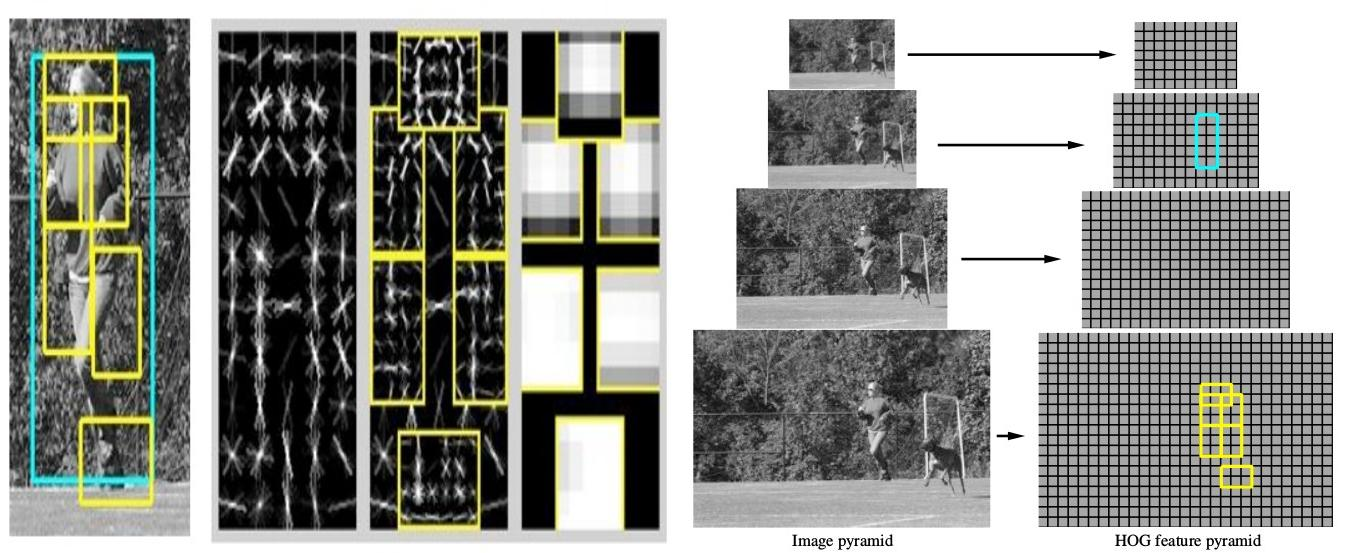
\includegraphics[scale=0.3]{{Images/chap4Fels}.jpg}}
  \caption{Ενδιάμεσα στάδια κατά την εφαρμογή της μεθόδου των Μοντέλων Παραμορφώσιμων Τμημάτων. $\textbf{Αριστερά}$: Το μοντέλο για την ανίχνευση ανθρώπων. Στο σχήμα φαίνονται τα σταθερά μέρη του ανθρώπου (άκρα και σώμα) τα οποία μπορούν να κινούνται σχετικά και να παραμένουν ενωμένα με χαλαρούς συνδέσμους. Ακόμα, βλέπουμε την απεικόνιση του μοντέλου στο πεδίο των περιγραφητών HOG και τα μέρη του όταν αναλυθούν. $\textbf{Δεξιά}$: Η κάθε εικόνα αναλύεται σε πολλαπλές κλίμακες έτσι ώστε να ενσωματώσει την πληροφορία του μεγέθους. Βλέπουμε πώς η πυραμίδα στο επίπεδο των κλιμάκων εικόνων μεταφέρεται στο χώρο χαρακτηριστικών HOG. Εικόνα από το \cite{felzenszwalb_2008}.}
  \label{fig:chap4Fels}
\end{figure}

\par Η μέθοδος εκκινεί με την εξαγωγή τοπικών χαρακτηριστικών τύπου HOG και μειώνει τη διάσταση με Ανάλυση Πρωταρχικών Συνιστωσών (PCA). Στη συνέχεια, χρησιμοποιεί τη μέθοδο «κυλιόμενου παραθύρου» για τις θέσεις του φίλτρου ρίζας σε κάθε κλίμακα. Τα φίλτρα τμημάτων εφαρμόζονται σε δύο κλίμακες υψηλότερης ανάλυσης και σε συντεταγμένες σχετικές ως προς τη θέση του φίλτρου ρίζας. Κάθε συνδυασμός θέσεων φίλτρων και κλίμακας αποκτά ένα σκορ, το οποίο υποθέτωντας $n$ φίλτρα τμημάτων δίνεται από την εξίσωση

\begin{equation}\label{eq:DPM}
    score(p_0,p_1, \dots ,p_P)=\sum_{i=0}^{n} F_i*\phi(H,p_i)-\sum_{i=1}^{n} d_i*\phi_d(dx_i,dy_i)+b
\end{equation}

Στην παραπάνω εξίσωση, $p_i$ είναι ο συμβολισμός του μέρους $i$, με το $p_0$ να δηλώνει τη ρίζα. Ο πρώτος όρος αποτελεί το άθροισμα των σκορ της εφαρμογής κάθε φίλτρου $F_i$ του τμήματος $p_i$ πάνω στη συνάρτηση απόδοσης σκορ για την κλίμακα $H$, που έχει σχηματιστεί κατά την εκπαίδευση. Όσο υψηλότερη τιμή λαμβάνει το άθροισμα αυτό, τόσο πιο βέβαιοι είμαστε για μια έγκυρη ανίχνευση. Ο δεύτερος όρος, ο οποίος αφαιρείται από τα σκορ ανίχνευσης, είναι τα κόστη παραμόρφωσης. Αν δηλαδή $d_i$ είναι η σχετική μετατόπιση του $p_i$ ως προς τη θέση που κατέχει το $p_i$ στο μοντέλο ρίζας που έχει τοποθετηθεί στη θέση που εξετάζουμε, $\phi_d$ είναι η συνάρτηση κόστους για μια τέτοια μετατόπιση, τότε το γινόμενο είναι το κόστος παραμόρφωσης και τείνει να επιβαρύνει υψηλές παραμορφώσεις από το μοντέλο που έχει προκύψει από την εκπαίδευση. Στην αυθεντική έκδοση της εργασίας, οι συναρτήσεις $\phi$ υλοποιούνται με Μηχανές Διανυσμάτων Υποστήριξης (SVM). Τέλος ο όρος $b$, είναι απλά ένα bias. Κρατάμε το μέγιστο της συνάρτησης αυτής πάνω στα $p_i $για όλες τις m-συνιστώσες. Υψηλό σκορ ρίζας για μια περιοχή μέσω της συνάρτησης αυτής ενδεικνύει το αντικείμενο. Μια μετεπεξεργασία η οποία περιλαμβάνει καταπίεση μη μεγίστων επιστρέφει το βέλτιστο ορθογώνιο ανίχνευσης.

\par Συμπερασματικά, η μέθοδος των DPM μπορεί να μοντελοποιήσει πολύπλευρες προκλήσεις που καθιστούν την ανίχνευση αντικειμένων ένα δύσκολο πρόβλημα. Άλλο βασικό πλεονέκτημα της μεθόδου είναι η υλοποίησή της με χρήση δυναμικού προγραμματισμού και γενικευμένων μετασχηματισμών απόστασης, στοιχείο που την καθιστά αρκετά γρήγορη. Φυσικά είναι πιο αργή από το ταίριασμα προτύπων αλλά ταυτόχρονα γενικεύει υπερβολικά καλύτερα. Σε επόμενη εργασία \cite{felzenszwalb_2010_cascade}, η ταχύτητα της μεθόδου αυξήθηκε δραματικά, δίνοντας περισσότερο μέγεθος στη δημοτικότητά της.


%%%%%%%%%%%%%%%%%%%%%%%%%%%%%%%%%%%%%%%%%%%%%%%%%%%%%% Our Approach
\section{Προτεινόμενο Σύστημα}
%%%%%%%%%%%%%%%%%%%%%%%%%%%%%%%% Dataset
\subsection{Το Σύνολο Δεδομένων για Ανίχνευση Αντικειμένων}
Το σύνολο δεδομένων που χρησιμοποιούμε παρέχει (στην νεότερή του μορφή) επισημειώσεις για σχέσεις αντικειμένων-ρημάτων ανά τμήμα που έχει κατηγοριοποιηθεί σε κάποια από τις κατηγορίες ρημάτων. Ωστόσο δεν παρέχει καμία επισημείωση για την όψη ή τη δομή των αντικειμένων αυτών. Οπότε για το πρόβλημα της ανίχνευσης αντικειμένων προβήκαμε σε δικές επισημειώσεις. Κατά τη διαδικασία αυτή διαπιστώσαμε προκλήσεις που υποθάλπουν στο σύνολο δεδομένων αυτό σχετικά με την ανίχνευση αντικειμένων και τις οποίες αναφέρουμε εδώ:

\begin{itemize}
  \item Συμβαίνουν συχνές, μερικές ή ολικές επικαλύψεις του αντικειμένου με άλλα αντικείμενα αλλά κυρίως με μέρη του ανθρώπινου σώματος, ιδιαίτερα χέρια.
  \item Η απόσταση από τη σταθερή κάμερα είναι μεγάλη για αναγνώριση αντικειμένων τέτοιου μεγέθους (όπως κομμένα λαχανικά ή μικρά μαγειρικά εργαλεία) με ακρίβεια.
  \item Υπάρχει μικρή μεταβλητότητα μεταξύ των διαφόρων κλάσεων αντικειμένων, όπως διάκριση μεταξύ παρόμοιων εμφανισιακά φρούτων σε μορφή κύβων.
  \item Ταυτόχρονα, υπάρχει μεγάλη μεταβλητότητα μεταξύ αντικειμένων της ίδιας κλάσης, όπως τα διαφορετικά είδη δοχείων.
  \item Υπάρχουν αντικείμενα τα οποία σχετίζονται με περιοχές του χώρου και δεν μπορούν να μοντελοποιηθούν επαρκώς, όπως ψυγείο, ντουλάπια και συρτάρια.
  \item Ακόμα πιο δύσκολα, υπάρχουν αντικείμενα τα οποία αλλάζουν σύσταση ή δομή κατά τη διάρκεια του βίντεο, αλλά συνεχίζουν να κατηγοριοποιούνται με την ίδια ετικέτα. Για παράδειγμα, φρούτα τα οποία από ακέραια μορφή κόβονται και στη συνέχεια πολτοποιούνται.
  \item Η έλλειψη πρότερης γνώσης για τα αντικείμενα που θα εμφανιστούν. Παρότι το λεξιλόγιο που χρησιμοποιούμε είναι περιορισμένο, συχνά εμφανίζονται συσκευασίες αγνώστου περιεχομένου, όπως μπουκάλια ή κουτιά.
  \item Η ανεπάρκεια γενικού μοντέλου για τα αντικείμενα της ίδιας κλάσης σε διαφορετικά βίντεο. Παρότι η πρόκληση αυτή είναι άμεσα συνδεδεμένη με την υψηλή ενδομεταβλητότητα, εν τούτοις αναφέρεται ξεχωριστά για να τονίσει τις διαφορές στις συνθήκες λήψης, όπως ο διαφορετικός φωτισμός, αλλά και τις δομικές διαφοροποιήσεις λόγω διαφορετικής επεξεργασίας των αντικειμένων σε διαφορετικά βίντεο.
\end{itemize}

\begin{figure}
  \centering
  \noindent\makebox[\textwidth]{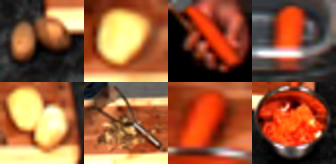
\includegraphics[scale=0.7]{{Images/chap4ObjDiff}.png}}
  \caption{Παρά την αλλαγή στη δομή και στη φύση τους, τα αντικείμενα συχνά εκπροσωπούνται από την ίδια ετικέτα κλάσης. Για παράδειγμα, μια πατάτα μπορεί να κοπεί σε κομμάτια, τα οποία διατηρούν την ιδιότητα της πατάτας. Ομοίως και μια σαλάτα καρότων, εντάσσεται στην κατηγορία καρότων. Τέτοιες διενέξεις στην εμφάνιση και την ετικέτα συμβαίνουν συχνά στο σύνολο δεδομένων που χρησιμοποιείται σε αυτή την εργασία, γεγονός που δυσχεραίνει σημαντικά τον εντοπισμό και την παρακολούθηση των αντικειμένων στη διάρκεια του βίντεο.}
  \label{fig:chap4ObjDiff}
\end{figure}

\par Ιδιαίτερη αναφορά αξίζει να γίνει για έναν παράγοντα που δυσκολεύει σημασιολογικά την έγκυρη γενική ανίχνευση αντικειμένων στα frames, τη χρήση των αντικειμένων. Ας σκεφτούμε για παράδειγμα ένα χώρο μαγειρικής όπου διάφορα υλικά και εργαλεία βρίσκονται πάνω σε ένα πάγκο. Ο δράστης στο βίντεο αλληλεπιδρά με ορισμένα από αυτά, τα οποία πρέπει να εντοπιστούν. Ωστόσο εδώ εμφανίζονται τα εξής προβλήματα. Αρχικά, ο πάγκος μπορεί να περιέχει πληθώρα αντικειμένων τα οποία επίσης θα ανιχνευτούν αλλά δε θα πρέπει να ληφθούν υπόψιν στη σημασιολογία καθώς δε χρησιμοποιούνται. Τώρα από τα αντικείμενα που χρησιμοποιούνται, τα εργαλεία (όπως το μαχαίρι) υπερκαλύπτονται από τα χέρια του δράστη ή τα άλλα χρησιμοποιούμενα αντικείμενα στα οποία εφαρμόζονται. Αυτό αποκλείει τη δυνατότητα εντοπισμού τους από ένα σύστημα που βασίζεται αποκλειστικά στην όραση. Από την άλλη, τα σκεύη που χρησιμοποιούνται μπορεί να παραμένουν ακίνητα (όπως ένα ταψί στο οποίο προσθέτουμε υλικά) και να μην φαίνεται η άμεση χρήση τους ή να χρησιμοποιούνται μόνο σε περιπτώσεις υψηλής κίνησης ή και αλληλεπίδρασης με τα χέρια και άρα υψηλής οπτικής μεταβλητότητας (όπως ένας τρίφτης). Όπως ήδη αναφέραμε εξάλλου, αντικείμενα όπως οι πρώτες ύλες αλλάζουν σύσταση και δομή κατά τη διάρκεια της δράσης. Τέλος, στις επισημειώσεις και στη σημασιολογία λαμβάνονται υπόψιν αντικείμενα τα οποία δεν μπορούμε να παρατηρήσουμε. Για παράδειγμα στη δράση “εξαγωγή από ψυγείο”, γνωρίζουμε ποια αντικείμενα συνδέονται σημασιολογικά, αλλά δεν μπορούμε να δούμε ποιο είναι το αντικείμενο που εξάγεται στη συγκεκριμένη περίπτωση παρά μόνο αφού εξαχθεί, οπότε έχει τελειώσει και η δράση. Θα δούμε στη συνέχεια πώς μοντελοποιούμε το πρόβλημα της ανίχνευσης αντικειμένων υπό αυτές τις δυσκολίες.


%%%%%%%%%%%%%%%%%%%%%%%%%%%%%%%%% ROI
\subsection{Η Εισαγωγή της Περιοχής Ενδιαφέροντος}
Τονίσαμε νωρίτερα τις δυσκολίες εντοπισμού των αντικειμένων σε εικόνες όπως τα frames του βίντεο. Καταλήξαμε στο ότι πέρα από τις προκλήσεις που ενέχει η ανίχνευση αυτή καθαυτή, πρέπει σημασιολογικά να καταλήξουμε στο αν ένα αντικείμενο χρησιμοποιείται στη διάρκεια μιας δράσης. Επιπλέον, πρέπει να αποφανθούμε για τον εντοπισμό αντικειμένων τα οποία δεν είναι οπτικά ευδιάκριτα. Στο σημείο αυτό θα προχωρήσουμε σε μια παραδοχή η οποία, παρότι ασθενής, μπορεί να συρρικνώσει αρκετά τις περιοχές μελέτης. Η παραδοχή αυτή αφορά το σχηματισμό περιοχών ενδιαφέροντος οι οποίες περιλαμβάνουν άνθρωπο ή αποτελούν προσκήνιο. Ο διαχωρισμός σε περιοχές είναι σύμφωνος με την διαίσθησή μας: πρώτα, η δράση εκτελείται από άνθρωπο, άρα είναι  βέβαιο ότι κοντά στα αντικείμενα δράσης θα βρίσκεται ο δράστης. Έπειτα, η δράση συνήθως σχετίζεται με κίνηση, οπότε το να ορίσουμε το προσκήνιο ως χώρο δράσης είναι μια κίνηση προς τη σωστή κατεύθυνση.

\par Σε περισσότερη λεπτομέρεια, χρησιμοποιούμε τον ανιχνευτή του \cite{felzenszwalb_2010} για ανίχνευση του ανθρώπου, προεκπαιδευμένο στο PASCAL VOC 2007 γνωρίζοντας εκ των προτέρων ότι μόνο ένας άνθρωπος θα εμφανίζεται στο βίντεο. Τρέχουμε τον ανιχνευτή ανθρώπων ανά 10 frames (περίπου 0.35 δευτερόλεπτα) υποθέτοντας ότι σε εργασίες μαγειρικής οι κινήσεις του δράστη θα είναι περιορισμένες στο χώρο και με μικρή σχετικά ταχύτητα, οπότε η θέση του δε θα αλλάζει σημαντικά στα 10 αυτά frames. Έτσι, θεωρούμε για τα 10 αυτά frames ταυτόσημα αποτελέσματα ανίχνευσης. Σε frames όπου ο ανιχνευτής αποτυγχάνει να εντοπίσει περιοχή ανθρώπου, εξισώνουμε την περιοχή ανθρώπου με αυτή της τελευταίας ανίχνευσης. Στην ειδική περίπτωση που ο ανιχνευτής δώσει κενή έξοδο στο πρώτο frame, θεωρούμε ότι ακόμα δεν έχει εισέλθει ο άνθρωπος κι έτσι αφήνουμε κενό το αποτέλεσμα. Σε frames όπου ο ανιχνευτής δώσει περισσότερες από μία περιοχές ανθρώπου, λαμβάνουμε το ελάχιστο ορθογώνιο που περικλείει την ένωση των περιοχών αυτών.

\par Για ανίχνευση προσκηνίου χρησιμοποιούμε μοντέλα GMM. Το αποτέλεσμα είναι συνήθως ένα σύνολο περιοχών τις οποίες συνενώνουμε και πάλι όπως και στην περίπτωση των περιοχών ανθρώπου. Ο αλγόριθμος ανίχνευσης προσκηνίου τρέχει όλα τα frames του βίντεο και αρχικοποιεί ένα μοντέλο παρασκηνίου από τα Ν πρώτα frames του βίντεο, ενώ δεν γίνεται ειδική διαχείριση των frames στα οποία έχουμε κενό αποτέλεσμα ανίχνευσης. Η μεταβλητή Ν είναι ρυθμιζόμενη παράμετρος και η τιμή της επιλέχθηκε ξεχωριστά για κάθε βίντεο (από 30 ως 95), ως συνάρτηση του συνολικού μήκους του βίντεο αλλά και του μήκους του αρχικού τμήματος βίντεο πριν την είσοδο του ανθρώπου και την εκκίνηση των δράσεων. Επιπλέον, καθορίστηκε η τιμή της παραμέτρου ρυθμού μάθησης στην τιμή 0.003, ώστε να δίνουμε χρονικό περιθώριο στην εξέλιξη δράσεων στις οποίες ο δράστης διατηρεί μεγάλο μέρος του σώματός του σταθερό. Τέτοιου είδους δράσεις εμφανίζονται συχνά στο σύνολο δεδομένων μας καθώς συχνά έχουμε εργασίες λεπτομέρειας όπου μόνο τα άκρα των χεριών κουνιούνται, όπως ο τεμαχισμός ενός φρούτου σε φέτες. Τέλος, επιλέγουμε ως ελάχιστο εμβαδόν μιας υποψήφιας περιοχής προσκηνίου τα 250 τετραγωνικά pixels.

\par Για την εξαγωγή των περιοχών ενδιαφέροντος, έχοντας το πολύ μία περιοχή ανθρώπου και το πολύ μία περιοχή προσκηνίου, προχωράμε αρχικά στη συνένωση αυτών των περιοχών. Αν και οι δύο περιοχές είναι κενές, τότε δεν υπάρχει περιοχή ενδιαφέροντος αφού μάλλον δεν υπάρχει άνθρωπος να δράσει. Σε διαφορετική περίπτωση, λαμβάνουμε και πάλι το ελάχιστο ορθογώνιο που περικλείει την ένωση των δύο περιοχών. Στη συνέχεια, επεκτείνουμε την περιοχή ενδιαφέροντος ως εξής: α) στον άξονα x, διευρύνουμε κατά 15 pixels το μέγιστο αριστερά και δεξιά, όπου αυτό είναι δυνατό και β) στον άξονα y, αφήνουμε την περιοχή ενδιαφέροντος να επεκταθεί σε όλο το ύψος της εικόνας ώστε να μπορεί συμπεριλάβει αντικείμενα σε όλο το ύψος, από τον πάγκο και τα αντικείμενα επί αυτού μέχρι τα ψηλότερα ντουλάπια.

\begin{figure}
  \centering
  \noindent\makebox[\textwidth]{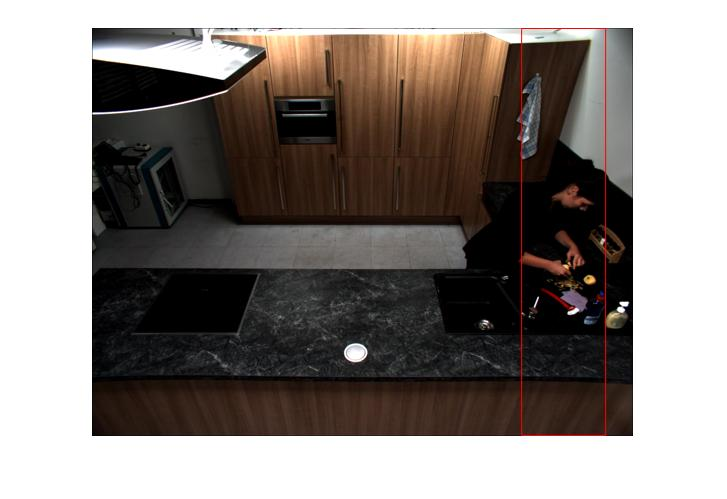
\includegraphics[scale=0.5]{{Images/chap4ROI}.jpg}}
  \caption{Ένα παράδειγμα εξαγωγής περιοχής ενδιαφέροντος. Σε πρώτη φάση τρέχουμε ανιχνευτή ανθρώπων βασισμένο σε DPM. Σε δεύτερη φάση, τρέχουμε ανίχνευση προσκηνίου με GMM. Συνενώνουμε το πλήθος των περιοχών που προκύπτουν σε όλη τους την έκταση. Επεκτείνουμε την περιοχή ενδιαφέροντος κατά ένα μικρό αριθμό πίξελ δεξιά και αριστερά, ενώ την αφήνουμε να λάβει όλο το ύψος της εικόνας. Έτσι μπορούμε να συλλάβουμε τμήματα αντικειμένων χώρου τα οποία μας βοηθούν στην ανίχνευσή τους όταν χρειάζεται, χωρίς όμως να κείνται εντός της περιοχής προσκηνίου ή εύρεσης ανθρώπου.}
  \label{fig:chap4ROI}
\end{figure}

\par Κατά τη διαδικασία κατασκευής της περιοχής ενδιαφέροντος είναι φανερά τα πλεονεκτήματα που εισάγει αυτή η σχεδίαση. Συσχετίζει άνθρωπο, περιοχές και αντικείμενα ενδιαφέροντος, εκτείνεται και εξελίσσεται δυναμικά ώστε να μην αποκλείει αντικείμενα ενδιαφέροντος και υπολογίζεται σχετικά εύκολα υπολογιστικά. Ωστόσο, τόσο ο ορισμός της όσο και οι παραδοχές που τον συνοδεύουν αφήνουν χώρο για άλλες προκλήσεις. Ξεκινώντας από τη μεταχείριση της εξόδου του ανιχνευτή ανθρώπου και λαμβάνοντας υπόψιν την αραιή χρονικά ανίχνευση και τη μέθοδο παρεμβολής που χρησιμοποιούμε βλέπουμε ότι το κόστος μιας αποτυχίας ανίχνευσης μεταφέρει την παρελθοντική θέση στο μέλλον, κάτι το οποίο μπορεί να προκαλέσει αρκετά λανθασμένη εκτίμηση της θέσης του ανθρώπου. Δεδομένου ότι το μοντέλο ανιχνευτή που εφαρμόζεται είναι προεκπαιδευμένο, υπάρχει χώρος για ανεπαρκείς εκτιμήσεις. Ακόμα χειρότερα, το σφάλμα μιας λανθασμένης ανίχνευσης μπορεί να συσσωρεύεται καθώς η αποτυχία επαναλαμβάνεται σε διαδοχικά frames. Στην περίπτωση εύρεσης παραπάνω της μιας περιοχής ανθρώπου, η συνένωση των περιοχών μπορεί να περικλείει περιοχές εντελώς άσχετες με την πραγματική περιοχή και άρα λανθασμένη επέκταση της περιοχής ενδιαφέροντος. Το ίδιο αποτέλεσμα μπορεί να προκαλέσει η παρόμοια μεταχείριση των πολλαπλών περιοχών προσκηνίου, οι οποίες μπορεί να περιέχουν και σφάλματα λόγω μεταβολών σκίασης και φωτισμού. Ο χαμηλός ρυθμός μάθησης καθυστερεί την εκμάθηση νέου μοντέλου υποβάθρου και συνεισφέρει στο να μην απορρίπτει προσκήνιο το οποίο παραμένει σταθερό για μικρό χρονικό διάστημα. Αν από την άλλη μέρος του προσκηνίου χαρακτηριστεί ως παρασκήνιο, ο μικρός ρυθμός μάθησης δυσχεραίνει την επαναφορά του στο προσκήνιο. Τέλος, η συνένωση περιοχών ανθρώπου και προσκηνίου και η επέκταση του αποτελέσματος είναι κάπως αυθαίρετη.

\par Σίγουρα πολλά από τα παραπάνω ζητήματα μπορούν να μοντελοποιηθούν εναλλακτικά, με διαφορετικά πλεονεκτήματα και μειονεκτήματα. Σε αυτό το σημείο θα σταθούμε στη δύναμη της μοντελοποίησης που τελικά χρησιμοποιήσαμε μπροστά στα παραπάνω ζητήματα, τονίζοντας όμως ότι αυτά συνεχίζουν να υπάρχουν ως κίνδυνοι. Το μοντέλο ανιχνευτή έχει προεκπαιδευτεί σε ένα μεγάλο και γενικό σύνολο δεδομένων κι έτσι αναμένουμε να γενικεύει με ευρωστία. Οι πολλαπλές περιοχές ανίχνευσης συνήθως παρουσιάζουν πολύ υψηλό ποσοστό επικάλυψης, όπως διαπιστώνεται πειραματικά, οπότε η συνένωσή τους είναι ασφαλής. Η αποκοπή μέρους του προσκηνίου δεν επηρεάζει σημαντικά το αποτέλεσμα καθώς η ένωση με την αρκετά ευρύτερη περιοχή ανθρώπου θα διατηρήσει την περιοχή ενδιαφέροντος πρακτικά αναλλοίωτη. Εξάλλου, αποκοπή προσκηνίου μπορεί να συμβεί σε περίπτωση μακράς σε χρονικό μήκος ακινησίας του δράστη, άρα το αποτέλεσμα της ανίχνευσης ανθρώπου θα είναι πρακτικά σταθερό. Τέλος, η επέκταση των περιοχών ενδιαφέροντος είναι η μόνη λύση για να εντοπίσουμε και αντικείμενα με τις δυσκολίες ανίχνευσης που έχουν αναφερθεί νωρίτερα. Αν και δεν είναι μαθηματικά φορμαλισμένη, η χρήση αυτής της επέκτασης μπορεί να αποδίδει πειραματικά, να περιλαμβάνει γειτονικά και χρήσιμα στη δράση αντικείμενα αλλά και να αποκόπτει ταυτόχρονα παρευρισκόμενα αλλά μη χρησιμοποιούμενα αντικείμενα.


%%%%%%%%%%%%%%%%%%%%%%%%%%%%%%%%% Object Detection
\subsection{Η Ανίχνευση Αντικειμένων}
Όπως σε κάθε πρόβλημα ανίχνευσης αντικειμένων, έτσι και σε αυτή την εργασία, προκειμένου να επιλέξουμε τον κατάλληλο ανιχνευτή πρέπει να ορίσουμε τις επιθυμητές προδιαγραφές, να εξετάσουμε ενδελεχώς το πώς οι δυσκολίες του συνόλου δεδομένων πρέπει να μοντελοποιηθούν αποτελεσματικά και να προβούμε στους απαραίτητους συμβιβασμούς. Νωρίτερα παρουσιάσαμε τις ιδιαιτερότητες του συνόλου δεδομένων που χρησιμοποιήσαμε σχετικά με την ανίχνευση αντικειμένων. Θα δείξουμε τώρα τη δική μας προσέγγιση και στη συνέχεια το πώς οι επιλογές που κάναμε στη σχεδίαση ανταποκρίνονται στις προκλήσεις του συνόλου δεδομένων.

\par Αρχικά, προβήκαμε σε ανίχνευση αντικειμένων ξεχωριστά στα frames και επιλέξαμε ανιχνευτή Ταιριάσματος Προτύπων με χρήση Αθροίσματος Τετραγωνικών Διαφορών (SSD) και τρέξαμε δειγματοληπτώντας το βίντεο ανά 10 frames, ως ένα συνδυασμό ταχύτητας και κάποιας ευρωστίας. Για κάθε βίντεο, εξαγάγαμε πρότυπα για ένα υποσύνολο των αντικειμένων τα οποία εμφανίζονται στο βίντεο. Τα αντικείμενα τα οποία επιλέχθηκαν για αναπαράσταση μέσω προτύπων ήταν αυτά τα οποία εμφανίζονταν σε αρκετά διαδοχικά frames με σταθερή μορφή και δυνατότητα αναπαράστασης. Για παράδειγμα, ένα φρούτο που κείται για κάποια δευτερόλεπτα στον πάγκο ακίνητο, μπορεί να εντοπισθεί αποτελεσματικά. Επιπλέον, αντικείμενα όπως το ψυγείο, οι ντουλάπες και τα συρτάρια, αναπαρίστανται από το μέρος του επίπλου που εμφανίζεται μόλις αυτά χρησιμοποιηθούν (ανοίξουν). Από την άλλη, αντικείμενα δυσδιάκριτα, όπως ένα μαχαίρι ή συνεχώς κινούμενα αντικείμενα, όπως μια κουτάλα, δεν αναπαρίστανται οπτικά καθώς δεν αρκεί μια εικόνα για να εντοπισθούν σε μεγάλη διάρκεια βίντεο. Περαιτέρω, σε κάθε βίντεο, μπορεί να χρησιμοποιούνται περισσότερα του ενός πρότυπα για την ίδια κατηγορία αντικειμένων. Μάλιστα για κάθε βίντεο γίνεται διαφορετική αναπαράσταση για την ίδια κατηγορία αντικειμένων, δηλαδή δεν χρησιμοποιούμε το ίδιο πρότυπο για πολλά βίντεο. Τέλος, αποφεύχθηκε η αναπαράσταση σταθερών χωρικών αντικειμένων, όπως εστία μαγειρέματος ή θήκη δοχείων μπαχαρικών, καθώς ο συνεχής τους εντοπισμός μας είναι άχρηστος αφού εμφανίζονται στα περισσότερα frames όμως συχνά δεν επηρεάζουν τη δράση λόγω της εμφάνισής τους και μόνο.

\begin{figure}
  \centering
  \noindent\makebox[\textwidth]{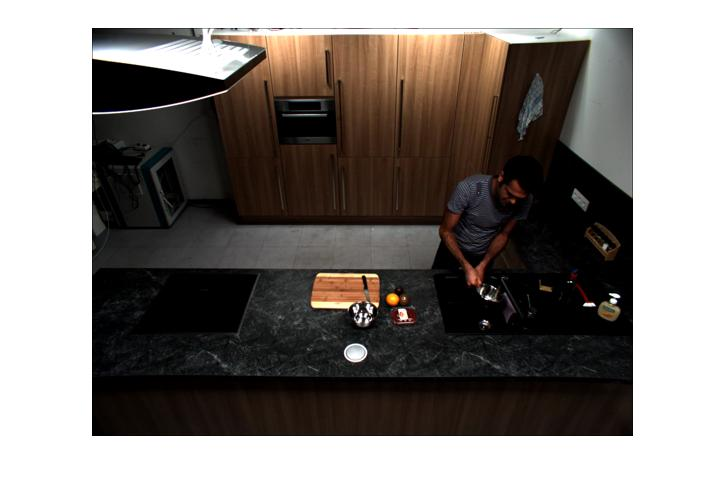
\includegraphics[scale=0.5]{{Images/chap4ROI2}.jpg}}
  \caption{Η οπτική ανίχνευση αντικειμένων μπορεί εύκολα να λειτουργήσει αποτελεσματικά, με τη μέθοδο Ταιριάσματος Προτύπων ή άλλη, σε εικόνες όπου γνωστά αντικείμενα κείνται ακίνητα και πρακτικά χωρίς επικαλύψεις. Εν τούτοις, μόνο η οπτική πληροφορία εισάγει με μεγάλη πιθανότητα σφάλματα μη χρήσης. Στην εικόνα, μπορούμε εύκολα να διακρίνουμε αντικείμενα όπως φρούτα και μαχαίρι πάνω στον πάγκο, ωστόσο ο δράστης δεν τα χρησιμοποιεί. Η πληροφορία ανίχνευσης αυτών των αντικειμένων είναι θόρυβος που επιβαρύνει τον τελικό ταξινομητή σημασιολογίας. Το πρόβλημα λύνεται με την εισαγωγή της περιοχής ενδιαφέροντος, χάρη στην οποία διαπιστώνουμε ότι τα εντοπιζόμενα αντικείμενα δεν βρίσκονται στην περιοχή προσκηνίου και άρα δε λαμβάνονται υπόψιν.}
  \label{fig:chap4ROI2}
\end{figure}

\par Θα σταθούμε εδώ για να αφουγκραστούμε τα πλεονεκτήματα που έχει μια τέτοια επιλογή δεδομένων των ιδιαιτεροτήτων του συνόλου δεδομένων. Η απόσταση από την κάμερα, παράγοντας που δυσχεραίνει την ανίχνευση των αντικειμένων, πλέον δεν επηρεάζει: έχουμε να ανιχνεύσουμε ένα σταθερό πρότυπο κι όχι να επισημάνουμε ακριβώς μια περιοχή του χώρου χωρίς πρότερη πληροφορία. Η αυστηρή ανίχνευση προτύπων μπορεί να αντισταθμίσει την χαμηλή μεταβλητότητα μεταξύ των διαφορετικών κλάσεων. Προς αυτή την κατεύθυνση, χρησιμοποιούμε αυστηρό κατώφλι στην έξοδο του SSD συστήματος, ίσο με 0.99. Το κατώφλι αυτό απορρίπτει ακόμα και παρόμοια αντικείμενα. Ωστόσο υπάρχει ο κίνδυνος να απορρίψει και διαφορετικές εμφανίσεις του ίδιου αντικειμένου υπό ελαφρά οπτική τροποποίηση. Το πρόβλημα αυτό αντιμετωπίζεται με την εξαγωγή περισσότερων από ένα προτύπων για το ίδιο αντικείμενο. Επίσης η στρατηγική αυτή προστατεύει από την υψηλή μεταβλητότητα μεταξύ αντικειμένων της ίδιας κατηγορίας ή ακόμα και την αλλαγή σύστασης των αντικειμένων: μια ακέραια ντομάτα και μια σάλτσα ντομάτας απεικονίζονται δικαίως ως διαφορετικά αντικείμενα αλλά αναφέρονται στην ίδια κλάση. Η επιλογή αναπαράστασης των αντικειμένων περιοχών (όπως το ψυγείο) με το μεταβλητό τους μέρος επιλύει και το ζήτημα μοντελοποίησής τους. Τέλος, με την χρήση διαφορετικών προτύπων ανά βίντεο, επιλύουμε και το ζήτημα μεταβλητότητας των αντικειμένων μεταξύ των βίντεο. Δηλαδή η επιλογή αυτού του μοντέλου αντικρούει 6 από τους 8 αναφερθέντες παράγοντες δυσκολίας ανίχνευσης.

\par Στη συνέχεια, εξετάζουμε το πρόβλημα της χρήσης. Είναι φανερό ότι σε κάθε δράση μας ενδιαφέρουν μόνο τα αντικείμενα που χρησιμοποιούνται στη διάρκειά της. Εν τούτοις, η χρήση των αντικειμένων, συχνότερα με τα χέρια, οδηγεί σε σημαντικές επικαλύψεις των αντικειμένων και τεράστια οπτική μεταβλητότητα. Η πρώτη απάντησή μας σε αυτό είναι η παρακολούθηση αντικειμένων τα οποία μπορούν να παραμένουν αναλλοίωτα ή να αναπαρίστανται από κάποιο σταθερό μέρος τους, π.χ. τα κομμάτια ενός φρούτου που κόβεται τα οποία έχουν ήδη κοπεί, παραμένουν σταθερά καθώς αυτό συνεχίζει να κόβεται. Η παρατήρηση οπτικά αναλλοίωτων αντικειμένων ωστόσο ενέχει άλλους κινδύνους: τα αντικείμενα αυτά μπορούν να εντοπίζονται σε ποικίλες χρονικές στιγμές χωρίς να αφορούν πραγματικά τη δράση. Αν, για παράδειγμα, ένα μαγειρικό σκεύος περιέχει φαγητό το οποίο βράζει πάνω στην εστία, ενώ ταυτόχρονα ο δράστης ασχολείται με μια άλλη εργασία, όπως προετοιμασία των υλικών που θα βράσουν, τότε το μαγειρικό σκεύος συνεχίζει να εντοπίζεται παρότι δεν αφορά τη δράση. Με άλλα λόγια, απαιτούμε από τον ανιχνευτή όχι απλά να εντοπίζει την εμφάνιση ή μη των αντικειμένων αλλά να λαμβάνει μια απόφαση σχετικά με το αν η εμφάνιση αυτή παρουσιάζει ενδιαφέρον για τη δράση. Για το λόγο αυτό, εισαγάγαμε την περιοχή ενδιαφέροντος, η κατασκευή της οποίας περιγράφηκε νωρίτερα. Κρατάμε ως ενδιαφέροντα τα αντικείμενα των οποίων το ορθογώνιο ανίχνευσης εμφανίζει μη κενή τομή με την περιοχή ενδιαφέροντος. Έτσι, περιμένουμε ότι στο προηγούμενο παράδειγμα, το μαγειρικό σκεύος δε θα περιέχεται στην περιοχή ενδιαφέροντος, στην οποία θα περιέχονται τα εργαλεία και τα υλικά που όντως αφορούν τη δράση. Φυσικά, υπάρχουν περιπτώσεις που αυτή η υπόθεση δεν επαληθεύεται, ειδικά αν λάβουμε υπόψιν την δειγματοληψία του βίντεο τόσο στην ανίχνευση αντικειμένων όσο και στην ανίχνευση ανθρώπων. Προς αυτή την κατεύθυνση, επιβάλλαμε περιορισμό στον συνολικό αριθμό των αναπαραστάσεων για κάθε αντικείμενο έτσι ώστε να ελαττώσουμε τις μη ενδιαφέρουσες ανιχνεύσεις.

\par Υπό τις παραπάνω παραδοχές και σχεδιαστικές επιλογές, τα αποτελέσματα ανίχνευσης είναι αρκετά εύρωστα και συνεπή. Μοντελοποιούνται ικανοποιητικά οι περισσότερες από τις προκλήσεις που εμφανίζει το σύνολο δεδομένων, ενώ αποκτούμε πληροφορία για τη χρησιμότητα της εμφάνισης στη δράση, μέσω της περιοχής ενδιαφέροντος. Ωστόσο, παρά τα προηγούμενα, εμφανίζονται ταυτόχρονα άλλα προβλήματα. Περιορίσαμε την ανίχνευση σε σχετικά σταθερά αντικείμενα με όριο στον αριθμό αναπαραστάσεων ανά αντικείμενο, αφήνοντας πολλαπλές εμφανίσεις αντικειμένων χωρίς αναπαράσταση. Ταυτόχρονα, το αυστηρό κατώφλι ταιριάσματος αποκλείει την ανίχνευση αντικειμένων χωρίς αναπαράσταση. Αναλογιζόμενοι αυτές τις δυσκολίες αξιοποιούμε επιπλέον αίσθηση για να ανιχνεύσουμε μεγαλύτερο εύρος αντικειμένων, μέσω της ομιλίας στο βίντεο.


%%%%%%%%%%%%%%%%%%%%%%%%%%%%%%%%%% Speech
\subsection{Η Αξιοποίηση της Ομιλίας στην Ανίχνευση Αντικειμένων}
Με την εισαγωγή της περιοχής ενδιαφέροντος θίξαμε τα ζητήματα ταυτοποίησης της χρήσης ή μη και του συσχετισμού των παρατηρούμενων αντικειμένων με τον δράστη. Μια άλλη τεχνική είναι να αξιοποιήσουμε τη συμπληρωματική φύση του λόγου και της οπτικής αντίληψης για να λάβουμε πληροφορία για τα χρησιμοποιούμενα αντικείμενα. Για το λόγο αυτό προβήκαμε στη δημιουργία υποτίτλων για τα βίντεο του test συνόλου δεδομένων. Η ιδέα είναι ότι η χρήση των υποτίτλων περιέχει πλούσια πληροφορία για τα αντικείμενα (εργαλεία και υλικά) που σχετίζονται άμεσα με τη δράση αλλά και για αντικείμενα τα οποία εμφανίζονται πρώτη φορά. Από τη γωνία του εντοπισμού αντικειμένων, ήδη γίνεται εμφανές το ότι τα δύο προβλήματα ανίχνευσης (με χρήση όρασης και με χρήση λόγου) είναι δυικά και συμπληρωματικά από τη φύση τους. Το πρώτο εστιάζει σε οπτικά αναλλοίωτα χαρακτηριστικά και εντοπίζει αντικείμενα που σχετίζονται με τη δράση χωρικά αλλά όχι άμεσα με το δράστη (πχ τα σκεύη, αλλά όχι τα εργαλεία), οπότε ένα τέτοιο σύστημα είναι εύρωστο σε αντικείμενα που παραμένουν ακίνητα αλλά χρήσιμα. Από την άλλη, ένα σύστημα εντοπισμού βασισμένο στο λόγο εστιάζει σε γλωσσικά αναλλοίωτα χαρακτηριστικά και τείνει να ανιχνεύει αντικείμενα που αναφέρονται συχνά και έχουν άμεση σχέση με το χρήστη, όπως τα εργαλεία και τα υλικά, τα οποία συνήθως έχουν άμεση αλληλεπίδραση με τα χέρια και παραμορφώνονται ή μεταβάλλονται δομικά.

\begin{figure}
  \centering
  \noindent\makebox[\textwidth]{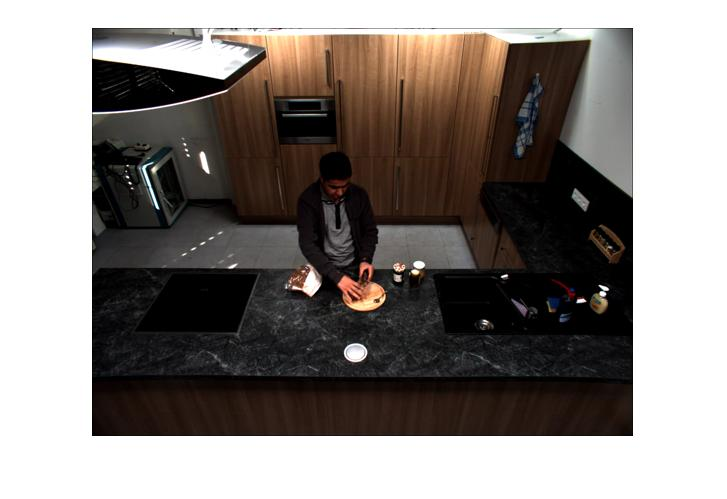
\includegraphics[scale=0.5]{{Images/chap4ROI3}.jpg}}
  \caption{Πολλές φορές η ανίχνευση αντικειμένων σε μια εικόνα είναι δυσεπίλυτο πρόβλημα ακόμα και για τον άνθρωπο. Δεν αρκεί μια εικόνα, κατά πάσα πιθανότητα, έτσι ώστε να συμπεράνουμε με ασφάλεια τι κρατάει στα χέρια του ο άνθρωπος της εικόνας. Σε αυτό μπορεί να συμβάλλει η εισαγωγή πρότερης γνώσης ή η ομιλία. Σε τέτοια βίντεο είναι αρκετά συχνή η συμπερίληψη των χρησιμοποιούμενων αντικειμένων στον λόγο. Συνδυάζοντας κατάλληλα λόγο και εικόνα λαμβάνουμε αρκετά πιο ισχυρές ενδείξεις για την εμφάνιση ενός αντικειμένου.}
  \label{fig:chap4ROI3}
\end{figure}

\par Η προσέγγιση εξαγωγής των εμφανίσεων των αντικειμένων γλωσσικά είναι αντίστοιχη με τη διαδικασία που εφαρμόστηκε στην περίπτωση της οπτικής ανίχνευσης. Αντί για την οπτική αμεταβλητότητα των σκευών ή αντικειμένων χώρου, εκμεταλλευόμαστε τη λεκτική αμεταβλητότητα των άμεσα χειριζόμενων αντικειμένων. Έτσι, υλοποιούμε ένα γλωσσικό template matching, αναζητώντας λέξεις κλειδιά μέσα στους υποτίτλους. Οι λέξεις αυτές ταυτίζονται με τις κλάσεις αντικειμένων του λεξιλογίου που χρησιμοποιούμε και η εμφάνιση μιας τέτοιας λέξης κατά μήκος ενός υποτίτλου αυτομάτως δηλώνει την ανίχνευση του αντικειμένου αυτού σε όλη τη διάρκεια του υποτίτλου. Επιπλέον, θεωρούμε συχνή τη χρήση κάποιου αντικειμένου και αφού έχει αναφερθεί, οπότε επεκτείνουμε το διάστημα μεταφράζοντας το παραπάνω εγχείρημα με χρήση ασαφούς λογικής: το αντικείμενο θα εμφανίζεται “τη στιγμή που αναφέρεται και λίγο μετά”. Τη φράση αυτή αποδίδει μια συνάρτησης μετοχής (η οποία μπορεί διαισθητικά να ληφθεί ως η εκ των υστέρων κατανομή της πιθανότητας εμφάνισης του αντικειμένου στο βίντεο ως προς το χρόνο, με δεδομένη την παρατήρηση του ονόματος κλάσης στον τρέχοντα υπότιτλο. Η συνάρτηση αυτή είναι μοναδιαία στο χρονικό διάστημα που ορίζει ο υπότιτλος, ενώ φθίνει γραμμικά μετά το χρονικό πέρας του υποτίτλου, μέχρι μηδενισμού, για χρονικό διάστημα ίσο με το 10\% της διάρκειας του υποτίτλου.


%%%%%%%%%%%%%%%%%%%%%%%%%%%%%% Fusion with speech
\subsection{Συνδυασμός Εικόνας και Γλώσσας}
Στα παραπάνω, τονίστηκε η συμπληρωματικότητα του λόγου και της οπτικής αντίληψης. Είναι φανερό ότι η μέγιστη ευρωστία αποκτάται συνενώνοντας τις δύο αυτές μεθόδους. Συνδυάζουμε τα αποτελέσματα ως εξής: Πρώτα, μετατρέπουμε τα αποτελέσματα οπτικής ανίχνευσης των αντικειμένων σε δυαδικά ιστογράμματα. Αυτό γίνεται ελέγχοντας τα frames στα οποία υπάρχει ορθογώνιο ανίχνευσης το οποίο περιέχεται έστω και μερικώς στην περιοχή ενδιαφέροντος και σημειώνοντας τιμή 1 για τα frames αυτά. Για αντικείμενα τα οποία αναπαρίστανται με περισσότερα από ένα πρότυπα, συνενώνουμε τα ιστογράμματα που προκύπτουν από την ανίχνευση των διαφορετικών προτύπων έτσι ώστε να έχουμε τιμή 1 αν έστω ένα από τα πρότυπα του αντικειμένου εντοπίσθηκε. Στη συνέχεια εξάγουμε τα ιστογράμματα από τους υποτίτλους, λαμβάνοντας υπόψιν την ασαφή συνάρτηση που πρέπει να εισάγουμε, οπότε εδώ δεν έχουμε δυαδικά ιστογράμματα. Αθροίζουμε τα παραπάνω ιστογράμματα (οπτικής ή γλωσσικής αντίληψης) για κάθε βίντεο και κλάση αντικειμένου. Είναι φανερό ότι τώρα θα έχουμε τιμές μεγαλύτερες της μονάδας. Ψαλιδίζουμε στο 1.1 κάθε τιμή μεγαλύτερη του 1.1. Με αυτόν τον τρόπο δίνουμε επιπλέον δύναμη στα frames όπου γλώσσα και όραση συμφωνούν αλλά, συγχρόνως, δεν τα αφήνουμε να έχουν τόση δύναμη ώστε να εκσφενδονίσουν οποιοδήποτε διάστημα στο οποίο συμμετέχουν σε μια τιμή που θα υποδηλώνει μεγάλη βεβαιότητα για την εμφάνιση του αντικειμένου σε όλο το διάστημά του.

\begin{figure}
  \centering
  \noindent\makebox[\textwidth]{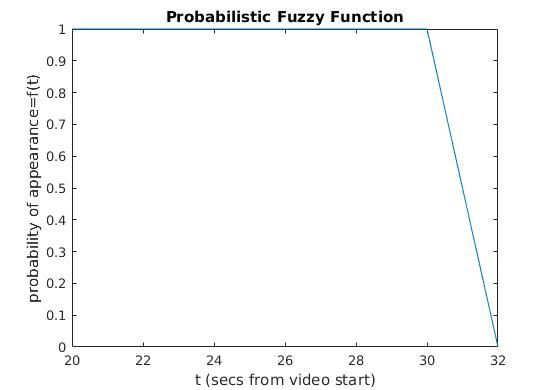
\includegraphics[scale=0.5]{{Images/chap4fuzzy}.jpg}}
  \caption{Θεωρούμε αυξημένη την πιθανότητα ένα αντικείμενο να εμφανίζεται "όσο διαρκεί ο υπότιτλος και λίγο μετά". Η φράση αυτή ερμηνεύεται μαθηματικά με μια ασαφή συνάρτηση μετοχής, η οποία έχει τιμή 1 στα χρονικά όρια του υποτίτλου και φθίνει γραμμικά μέχρι μηδενισμού από το πέρας του υποτίτλου μέχρι και 10\% της διάρκειάς του έπειτα από αυτόν. Για παράδειγμα, η συνάρτηση μετοχής για ένα αντικείμενο που αναφέρεται στον υπότιτλο στο χρονικό παράθυρο μεταξύ 20 και 30 δευτερολέπτων έχει τη μορφή της εικόνας.}
  \label{fig:chap4fuzyy}
\end{figure}

\par Τώρα για την αναπαράσταση ενός τμήματος βίντεο, λαμβάνουμε τα αθροιστικά ιστογράμματα πάνω στα frames που το αποτελούν. Προκύπτει ένα διάνυσμα όπου κάθε θέση περιέχει ένα αριθμό, που όσο μεγαλύτερος είναι τόσο πιο σίγουροι είμαστε για την εμφάνιση του αντικειμένου στο frame. Διαιρούμε το διάνυσμα με το μήκος του διαστήματος σε frames, λαμβάνουμε δηλαδή το μέσο ιστόγραμμα κατά μήκος του τμήματος βίντεο. Μετατρέπουμε το ιστόγραμμα σε δυαδικό επιλέγοντας κατώφλι 0.8. Το κατώφλι αυτό απορρίπτει λανθασμένες ευρέσεις αντικειμένων μέσα στην περιοχή ενδιαφέροντος, όπου ο όρος «λανθασμένες» εδώ, αφορά την αδιαφορία της εμφάνισης ως προς τη δράση, ενώ, ταυτόχρονα, ενισχύει τμήματα μεγάλης βεβαιότητας χωρίς αυτά να επισκιάζουν τμήματα μικρότερης βεβαιότητας. Τελικά λαμβάνουμε ένα δυαδικό διάνυσμα μήκους ίσο με το πλήθος των αντικειμένων του λεξιλογίου.

\par Πριν κλείσουμε το κεφάλαιο αυτό πρέπει να σχολιάσουμε δύο πράγματα. Αρχικά, σε θεωρητικό επίπεδο, θα δούμε πώς ο συνδυασμός γλώσσας και όρασης, μαζί με τις σχεδιαστικές μας επιλογές, οδήγησαν σε μια δυνατή μοντελοποίηση των δυσκολιών του συνόλου δεδομένων. Οι 8 απαριθμημένες προκλήσεις που αφορούν την οπτική αντίληψη δεν επηρεάζουν τη γλωσσική αντίληψη, αλλά είδαμε πώς, ακόμα και μέσω της οπτικής αντίληψης, αντιμετωπίσθηκαν δυσκολίες όπως η μεταβλητότητα, η απόσταση από την κάμερα, η αναπαράσταση χώρων και η αλλαγή δομής των αντικειμένων στο χρόνο. Παράλληλα, η χρησιμότητα των εμφανίσεων προσεγγίστηκε με την χρήση της περιοχής ενδιαφέροντος, ενώ το άθροισμα των γλωσσικών και οπτικων ιστογραμμάτων μπορεί να αντισταθμίζει λάθη του ενός από τα δύο συστήματα. Το άλλο θέμα στο οποίο πρέπει να σταθούμε είναι, σε πειραματικό επίπεδο, να αξιολογήσουμε την απόδοση της ανίχνευσης αντικειμένων ανά τμήμα ενδιαφέροντος. Το πρόβλημα αυτό είναι any-of, δηλαδή κάθε τμήμα μπορεί να ανήκει σε πολλές κατηγορίες ταυτόχρονα, με άλλα λόγια στο πρόβλημά μας, κάθε τμήμα να περιέχει πολλά από τα αντικείμενα. Οπότε θα χρησιμοποιήσουμε μετρικές multilabel ταξινομητών. Ως ground truth λαμβάνουμε τις επισημειώσεις του MPII Cooking Dataset 2 για τα αντικείμενα που χρησιμοποιούνται σε κάθε δράση. Τα αποτελέσματα φαίνονται στον πίνακα \ref{tab:ObjeResult}.

\begin{table}
	\centering
    \begin{tabular}{| l | l | l | l |}
    \hline
    \textbf{Metric} & \textbf{Value} \\ \hline
    Accuracy & 77.95\% \\ \hline
    Recall & 0.91 \\ \hline
    Precision & 0.87 \\ \hline
    F1-score & 0.88 \\
    \hline
    \end{tabular}
	\caption{Αποτελέσματα 4 μετρικών για την ανίχνευση αντικειμένων πάνω σε όλα τα βίντεο του συνόλου δεδομένων test που χρησιμοποιήσαμε. Παρατηρούμε ότι με σύζευξη λόγου και εικόνας μπορούμε να πετύχουμε ικανοποιητικά αποτελέσματα, πολύ πιο εύρωστα από ό,τι με χρήση μόνο ενός από τους δύο τρόπους.}
	\label{tab:ObjeResult}
\end{table}

\par Τα παραπάνω αποτελέσματα και οι δυσκολίες που αντιμετωπίσθηκαν μας υποδεικνύουν κάποια συμπεράσματα για τη συνθετότητα της ανθρώπινης αντίληψης όταν μιλάμε για ανίχνευση αντικειμένων. Παρατηρώντας τη δυνατότητα του ανθρώπου να εντοπίζει τόσο εύκολα το αντικείμενο της επιλογής του σε μια εικόνα που δεν έχει ξαναδεί, πράγματι κανείς εντυπωσιάζεται αν αναλογισθεί πόσο δύσκολο υπολογιστικά πρόβλημα είναι. Εμείς στεκόμαστε στη δυνατότητα του ανθρώπου να αντιληφθεί τα αντικείμενα αυτού του συνόλου δεδομένων για να βγάλουμε κάποια πορίσματα και όχι σε ψυχοφυσικές έρευνες. Αρχικά, ο άνθρωπος δε χρησιμοποιεί μία αντίληψη μόνο για να εξάγει ένα συμπέρασμα. Υπάρχει πάντα πληροφορία από τα συμφραζόμενα αλλά και από παραμορφώσιμα μοντέλα για τη δομή του αντικειμένου. Η σημασιολογία είναι επίσης κάτι πρωτίστης σημασίας στη λήψη αποφάσεων. Στη δική μας περίπτωση, δυσδιάκριτα μαγειρικά μπορούν να διακριθούν από τη χρήση τους, το χειρισμό τους, αλλά και τη σύνδεση με άλλα υλικά. Μάλιστα η ανθρώπινη εμπειρία μπορεί να ανακατασκευάσει τμήματα του αντικειμένου σε εικόνες που αυτό επικαλύπτεται ακόμα και πλήρως, μόνο από τη σημασιολογία της δράσης. Ακόμα και το σενάριο μπορεί να εξαχθεί και να δώσει διαφορετική πρότερη πιθανότητα σε αντικείμενα που μπορούν να εμφανιστούν, μοντελοποιώντας έτσι την έλλειψη πρότερης γνώσης για τα αντικείμενα που εμφανίζονται πρώτη φορά. Τέλος, ο άνθρωπος αντιλαμβάνεται τη χρονική αλληλουχία και τα αποτελέσματα που αυτή επιφέρει. Με αυτόν τον τρόπο, μπορεί να γνωρίζει την ύπαρξη ενός αντικειμένου στο χώρο χωρίς να την αντιλαμβάνεται οπτικά. Ταυτόχρονα, αισθάνεται τις μεταβολές στη φύση των αντικειμένων και συχνά είναι σε θέση να τις προβλέψει από την αλληλεπίδρασή τους με τα άλλα αντικείμενα. Συνολικά, μια σχεδιαστική μέθοδος ταιριάσματος, όπως αυτή που επιλέξαμε, καθόλου δεν συνδέεται με τη μοντελοποίηση και τη συνθετότητα της ανθρώπινης αντίληψης, παρότι αποκρίνεται στις προκλήσεις του συνόλου δεδομένων και δίνει καλά αποτελέσματα.






\end{document}
